\documentclass[twoside]{book}

% Packages required by doxygen
\usepackage{calc}
\usepackage{doxygen}
\usepackage{graphicx}
\usepackage[utf8]{inputenc}
\usepackage{makeidx}
\usepackage{multicol}
\usepackage{multirow}
\usepackage{textcomp}
\usepackage[table]{xcolor}

% Font selection
\usepackage[T1]{fontenc}
\usepackage{mathptmx}
\usepackage[scaled=.90]{helvet}
\usepackage{courier}
\usepackage{amssymb}
\usepackage{sectsty}
\renewcommand{\familydefault}{\sfdefault}
\allsectionsfont{%
  \fontseries{bc}\selectfont%
  \color{darkgray}%
}
\renewcommand{\DoxyLabelFont}{%
  \fontseries{bc}\selectfont%
  \color{darkgray}%
}

% Page & text layout
\usepackage{geometry}
\geometry{%
  a4paper,%
  top=2.5cm,%
  bottom=2.5cm,%
  left=2.5cm,%
  right=2.5cm%
}
\tolerance=750
\hfuzz=15pt
\hbadness=750
\setlength{\emergencystretch}{15pt}
\setlength{\parindent}{0cm}
\setlength{\parskip}{0.2cm}
\makeatletter
\renewcommand{\paragraph}{%
  \@startsection{paragraph}{4}{0ex}{-1.0ex}{1.0ex}{%
    \normalfont\normalsize\bfseries\SS@parafont%
  }%
}
\renewcommand{\subparagraph}{%
  \@startsection{subparagraph}{5}{0ex}{-1.0ex}{1.0ex}{%
    \normalfont\normalsize\bfseries\SS@subparafont%
  }%
}
\makeatother

% Headers & footers
\usepackage{fancyhdr}
\pagestyle{fancyplain}
\fancyhead[LE]{\fancyplain{}{\bfseries\thepage}}
\fancyhead[CE]{\fancyplain{}{}}
\fancyhead[RE]{\fancyplain{}{\bfseries\leftmark}}
\fancyhead[LO]{\fancyplain{}{\bfseries\rightmark}}
\fancyhead[CO]{\fancyplain{}{}}
\fancyhead[RO]{\fancyplain{}{\bfseries\thepage}}
\fancyfoot[LE]{\fancyplain{}{}}
\fancyfoot[CE]{\fancyplain{}{}}
\fancyfoot[RE]{\fancyplain{}{\bfseries\scriptsize Generated on Mon Nov 18 2013 22\-:36\-:25 for W\-P-\/\-Engine by Doxygen }}
\fancyfoot[LO]{\fancyplain{}{\bfseries\scriptsize Generated on Mon Nov 18 2013 22\-:36\-:25 for W\-P-\/\-Engine by Doxygen }}
\fancyfoot[CO]{\fancyplain{}{}}
\fancyfoot[RO]{\fancyplain{}{}}
\renewcommand{\footrulewidth}{0.4pt}
\renewcommand{\chaptermark}[1]{%
  \markboth{#1}{}%
}
\renewcommand{\sectionmark}[1]{%
  \markright{\thesection\ #1}%
}

% Indices & bibliography
\usepackage{natbib}
\usepackage[titles]{tocloft}
\setcounter{tocdepth}{3}
\setcounter{secnumdepth}{5}
\makeindex

% Hyperlinks (required, but should be loaded last)
\usepackage{ifpdf}
\ifpdf
  \usepackage[pdftex,pagebackref=true]{hyperref}
\else
  \usepackage[ps2pdf,pagebackref=true]{hyperref}
\fi
\hypersetup{%
  colorlinks=true,%
  linkcolor=blue,%
  citecolor=blue,%
  unicode%
}

% Custom commands
\newcommand{\clearemptydoublepage}{%
  \newpage{\pagestyle{empty}\cleardoublepage}%
}


%===== C O N T E N T S =====

\begin{document}

% Titlepage & ToC
\hypersetup{pageanchor=false}
\pagenumbering{roman}
\begin{titlepage}
\vspace*{7cm}
\begin{center}%
{\Large W\-P-\/\-Engine \\[1ex]\large 0.\-1 }\\
\vspace*{1cm}
{\large Generated by Doxygen 1.8.5}\\
\vspace*{0.5cm}
{\small Mon Nov 18 2013 22:36:25}\\
\end{center}
\end{titlepage}
\clearemptydoublepage
\tableofcontents
\clearemptydoublepage
\pagenumbering{arabic}
\hypersetup{pageanchor=true}

%--- Begin generated contents ---
\chapter{Namespace Index}
\section{Namespace List}
Here is a list of all documented namespaces with brief descriptions\-:\begin{DoxyCompactList}
\item\contentsline{section}{\hyperlink{namespacewp__engine}{wp\-\_\-engine} }{\pageref{namespacewp__engine}}{}
\end{DoxyCompactList}

\chapter{Hierarchical Index}
\section{Class Hierarchy}
This inheritance list is sorted roughly, but not completely, alphabetically\-:\begin{DoxyCompactList}
\item \contentsline{section}{wp\-\_\-engine.\-Animation}{\pageref{classwp__engine_1_1_animation}}{}
\item \contentsline{section}{wp\-\_\-engine.\-Audio\-Handler}{\pageref{classwp__engine_1_1_audio_handler}}{}
\item \contentsline{section}{wp\-\_\-engine.\-Event}{\pageref{classwp__engine_1_1_event}}{}
\item \contentsline{section}{wp\-\_\-engine.\-Event\-Handler}{\pageref{classwp__engine_1_1_event_handler}}{}
\item \contentsline{section}{wp\-\_\-engine.\-Object}{\pageref{classwp__engine_1_1_object}}{}
\begin{DoxyCompactList}
\item \contentsline{section}{wp\-\_\-engine.\-Animated\-Object}{\pageref{classwp__engine_1_1_animated_object}}{}
\item \contentsline{section}{wp\-\_\-engine.\-Event\-Object}{\pageref{classwp__engine_1_1_event_object}}{}
\item \contentsline{section}{wp\-\_\-engine.\-Live\-Object}{\pageref{classwp__engine_1_1_live_object}}{}
\end{DoxyCompactList}
\item \contentsline{section}{wp\-\_\-engine.\-Slide\-Show}{\pageref{classwp__engine_1_1_slide_show}}{}
\item \contentsline{section}{wp\-\_\-engine.\-State\-Interface}{\pageref{interfacewp__engine_1_1_state_interface}}{}
\begin{DoxyCompactList}
\item \contentsline{section}{wp\-\_\-engine.\-State}{\pageref{classwp__engine_1_1_state}}{}
\begin{DoxyCompactList}
\item \contentsline{section}{wp\-\_\-engine.\-Help\-State}{\pageref{classwp__engine_1_1_help_state}}{}
\item \contentsline{section}{wp\-\_\-engine.\-Menu\-State}{\pageref{classwp__engine_1_1_menu_state}}{}
\end{DoxyCompactList}
\end{DoxyCompactList}
\item \contentsline{section}{wp\-\_\-engine.\-State\-Manager}{\pageref{classwp__engine_1_1_state_manager}}{}
\item \contentsline{section}{wp\-\_\-engine.\-Text}{\pageref{classwp__engine_1_1_text}}{}
\end{DoxyCompactList}

\chapter{Class Index}
\section{Class List}
Here are the classes, structs, unions and interfaces with brief descriptions\-:\begin{DoxyCompactList}
\item\contentsline{section}{\hyperlink{classwp__engine_1_1_animated_object}{wp\-\_\-engine.\-Animated\-Object} \\*A class for animated objects }{\pageref{classwp__engine_1_1_animated_object}}{}
\item\contentsline{section}{\hyperlink{classwp__engine_1_1_animation}{wp\-\_\-engine.\-Animation} \\*A class designed to simplify animations }{\pageref{classwp__engine_1_1_animation}}{}
\item\contentsline{section}{\hyperlink{classwp__engine_1_1_audio_handler}{wp\-\_\-engine.\-Audio\-Handler} \\*A class for handling the audio elements of the game }{\pageref{classwp__engine_1_1_audio_handler}}{}
\item\contentsline{section}{\hyperlink{classwp__engine_1_1_event}{wp\-\_\-engine.\-Event} \\*A class that contains all of the information of a single touch event required by the other partitions of the library }{\pageref{classwp__engine_1_1_event}}{}
\item\contentsline{section}{\hyperlink{classwp__engine_1_1_event_handler}{wp\-\_\-engine.\-Event\-Handler} \\*A class that simplifies touch event handling }{\pageref{classwp__engine_1_1_event_handler}}{}
\item\contentsline{section}{\hyperlink{classwp__engine_1_1_event_object}{wp\-\_\-engine.\-Event\-Object} \\*A class of event handling objects }{\pageref{classwp__engine_1_1_event_object}}{}
\item\contentsline{section}{\hyperlink{classwp__engine_1_1_help_state}{wp\-\_\-engine.\-Help\-State} \\*A class for help screens in games }{\pageref{classwp__engine_1_1_help_state}}{}
\item\contentsline{section}{\hyperlink{classwp__engine_1_1_live_object}{wp\-\_\-engine.\-Live\-Object} \\*A class for moving objects }{\pageref{classwp__engine_1_1_live_object}}{}
\item\contentsline{section}{\hyperlink{classwp__engine_1_1_menu_state}{wp\-\_\-engine.\-Menu\-State} \\*A class for menu screen in a game }{\pageref{classwp__engine_1_1_menu_state}}{}
\item\contentsline{section}{\hyperlink{classwp__engine_1_1_object}{wp\-\_\-engine.\-Object} \\*A class for graphical 2\-D objects }{\pageref{classwp__engine_1_1_object}}{}
\item\contentsline{section}{\hyperlink{classwp__engine_1_1_slide_show}{wp\-\_\-engine.\-Slide\-Show} \\*A class for multiple animation\-: a slideshow }{\pageref{classwp__engine_1_1_slide_show}}{}
\item\contentsline{section}{\hyperlink{classwp__engine_1_1_state}{wp\-\_\-engine.\-State} \\*The base class for all of the game states }{\pageref{classwp__engine_1_1_state}}{}
\item\contentsline{section}{\hyperlink{interfacewp__engine_1_1_state_interface}{wp\-\_\-engine.\-State\-Interface} \\*The inteface for game states }{\pageref{interfacewp__engine_1_1_state_interface}}{}
\item\contentsline{section}{\hyperlink{classwp__engine_1_1_state_manager}{wp\-\_\-engine.\-State\-Manager} \\*A class that handles the states smoothly }{\pageref{classwp__engine_1_1_state_manager}}{}
\item\contentsline{section}{\hyperlink{classwp__engine_1_1_text}{wp\-\_\-engine.\-Text} \\*A class for text elements }{\pageref{classwp__engine_1_1_text}}{}
\end{DoxyCompactList}

\chapter{Namespace Documentation}
\hypertarget{namespacewp__engine}{\section{Package wp\-\_\-engine}
\label{namespacewp__engine}\index{wp\-\_\-engine@{wp\-\_\-engine}}
}
\subsection*{Classes}
\begin{DoxyCompactItemize}
\item 
class \hyperlink{classwp__engine_1_1_animated_object}{Animated\-Object}
\begin{DoxyCompactList}\small\item\em A class for animated objects. \end{DoxyCompactList}\item 
class \hyperlink{classwp__engine_1_1_animation}{Animation}
\begin{DoxyCompactList}\small\item\em A class designed to simplify animations. \end{DoxyCompactList}\item 
class \hyperlink{classwp__engine_1_1_audio_handler}{Audio\-Handler}
\begin{DoxyCompactList}\small\item\em A class for handling the audio elements of the game. \end{DoxyCompactList}\item 
class \hyperlink{classwp__engine_1_1_event}{Event}
\begin{DoxyCompactList}\small\item\em A class that contains all of the information of a single touch event required by the other partitions of the library. \end{DoxyCompactList}\item 
class \hyperlink{classwp__engine_1_1_event_handler}{Event\-Handler}
\begin{DoxyCompactList}\small\item\em A class that simplifies touch event handling. \end{DoxyCompactList}\item 
class \hyperlink{classwp__engine_1_1_event_object}{Event\-Object}
\begin{DoxyCompactList}\small\item\em A class of event handling objects. \end{DoxyCompactList}\item 
class \hyperlink{classwp__engine_1_1_help_state}{Help\-State}
\begin{DoxyCompactList}\small\item\em A class for help screens in games. \end{DoxyCompactList}\item 
class \hyperlink{classwp__engine_1_1_live_object}{Live\-Object}
\begin{DoxyCompactList}\small\item\em A class for moving objects. \end{DoxyCompactList}\item 
class \hyperlink{classwp__engine_1_1_menu_state}{Menu\-State}
\begin{DoxyCompactList}\small\item\em A class for menu screen in a game. \end{DoxyCompactList}\item 
class \hyperlink{classwp__engine_1_1_object}{Object}
\begin{DoxyCompactList}\small\item\em A class for graphical 2\-D objects. \end{DoxyCompactList}\item 
class \hyperlink{classwp__engine_1_1_slide_show}{Slide\-Show}
\begin{DoxyCompactList}\small\item\em A class for multiple animation\-: a slideshow. \end{DoxyCompactList}\item 
class \hyperlink{classwp__engine_1_1_state}{State}
\begin{DoxyCompactList}\small\item\em The base class for all of the game states. \end{DoxyCompactList}\item 
interface \hyperlink{interfacewp__engine_1_1_state_interface}{State\-Interface}
\begin{DoxyCompactList}\small\item\em The inteface for game states. \end{DoxyCompactList}\item 
class \hyperlink{classwp__engine_1_1_state_manager}{State\-Manager}
\begin{DoxyCompactList}\small\item\em A class that handles the states smoothly. \end{DoxyCompactList}\item 
class \hyperlink{classwp__engine_1_1_text}{Text}
\begin{DoxyCompactList}\small\item\em A class for text elements. \end{DoxyCompactList}\end{DoxyCompactItemize}
\subsection*{Enumerations}
\begin{DoxyCompactItemize}
\item 
enum {\bfseries Layer} \{ {\bfseries B\-O\-T\-T\-O\-M}, 
{\bfseries M\-I\-D\-D\-L\-E}, 
{\bfseries T\-O\-P}
 \}
\item 
enum \hyperlink{namespacewp__engine_aae123481cdcc6dc4c4474c1b0b62b152}{state\-Identifier} \{ \\*
{\bfseries M\-E\-N\-U}, 
{\bfseries H\-E\-L\-P}, 
{\bfseries G\-A\-M\-E}, 
{\bfseries E\-X\-I\-T}, 
\\*
{\bfseries N\-O\-N\-E}
 \}
\begin{DoxyCompactList}\small\item\em Consists of identifiers for the most basic states. \end{DoxyCompactList}\end{DoxyCompactItemize}

\chapter{Class Documentation}
\hypertarget{classwp__engine_1_1_animated_object}{\section{wp\-\_\-engine.\-Animated\-Object Class Reference}
\label{classwp__engine_1_1_animated_object}\index{wp\-\_\-engine.\-Animated\-Object@{wp\-\_\-engine.\-Animated\-Object}}
}


A class for animated objects.  


Inheritance diagram for wp\-\_\-engine.\-Animated\-Object\-:\begin{figure}[H]
\begin{center}
\leavevmode
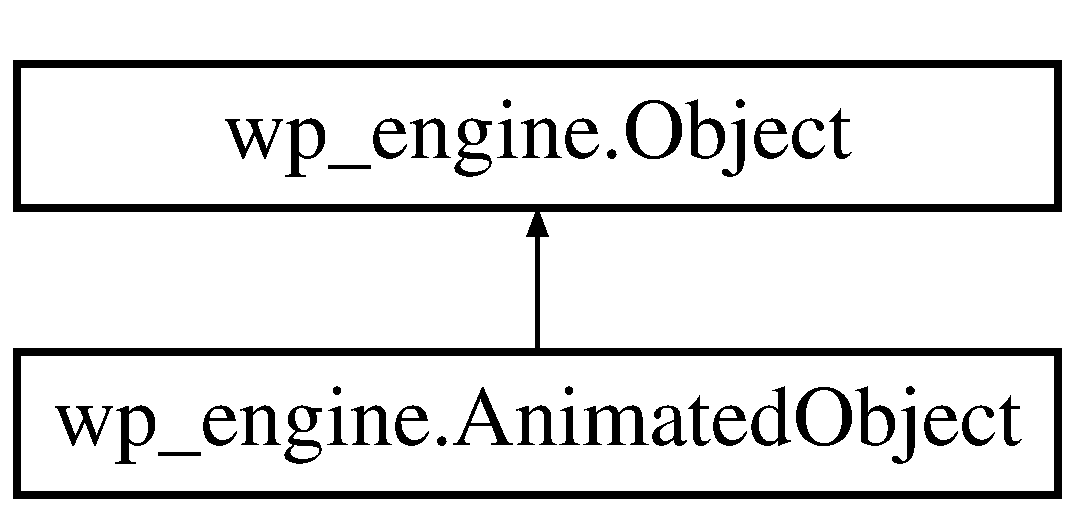
\includegraphics[height=2.000000cm]{classwp__engine_1_1_animated_object}
\end{center}
\end{figure}
\subsection*{Public Member Functions}
\begin{DoxyCompactItemize}
\item 
\hyperlink{classwp__engine_1_1_animated_object_a43b6d15d770384cafc4546b447a63303}{Animated\-Object} (float x, float y, Layer layer)
\begin{DoxyCompactList}\small\item\em A constructor. \end{DoxyCompactList}\item 
void \hyperlink{classwp__engine_1_1_animated_object_a4d244865b8e26ffbbd9f9f8658ff9d6b}{load\-Textures} (Content\-Manager content\-Manager, string folder\-Name)
\begin{DoxyCompactList}\small\item\em Loads the animation textures. \end{DoxyCompactList}\item 
void \hyperlink{classwp__engine_1_1_animated_object_a5cf1995b0821dcb47fd878adcd996257}{update} (float elapsed)
\begin{DoxyCompactList}\small\item\em Update function. \end{DoxyCompactList}\item 
void \hyperlink{classwp__engine_1_1_animated_object_ab14a6e72ab2ff3a3c3ffbbfc2aa152f8}{stop\-Animation} ()
\begin{DoxyCompactList}\small\item\em Stops the animation of the object. \end{DoxyCompactList}\item 
void \hyperlink{classwp__engine_1_1_animated_object_af25e7e5021799779dae6a46c23458f48}{start\-Animation} ()
\begin{DoxyCompactList}\small\item\em Starts the animation from the texture it was displaying previously. \end{DoxyCompactList}\item 
void \hyperlink{classwp__engine_1_1_animated_object_ac55ab9141a73b2e220934a01e36083c8}{reset\-Animation} ()
\begin{DoxyCompactList}\small\item\em Starts the animation from the beginning. \end{DoxyCompactList}\item 
float \hyperlink{classwp__engine_1_1_animated_object_aa14b0987cad18b3268fb3a1601d839a2}{get\-Animation\-Length} ()
\begin{DoxyCompactList}\small\item\em Return the length of the animation in seconds. \end{DoxyCompactList}\end{DoxyCompactItemize}
\subsection*{Additional Inherited Members}


\subsection{Detailed Description}
A class for animated objects. 

Part of the animation partition.

Inherits \hyperlink{classwp__engine_1_1_object}{Object}. 

\subsection{Constructor \& Destructor Documentation}
\hypertarget{classwp__engine_1_1_animated_object_a43b6d15d770384cafc4546b447a63303}{\index{wp\-\_\-engine\-::\-Animated\-Object@{wp\-\_\-engine\-::\-Animated\-Object}!Animated\-Object@{Animated\-Object}}
\index{Animated\-Object@{Animated\-Object}!wp_engine::AnimatedObject@{wp\-\_\-engine\-::\-Animated\-Object}}
\subsubsection[{Animated\-Object}]{\setlength{\rightskip}{0pt plus 5cm}wp\-\_\-engine.\-Animated\-Object.\-Animated\-Object (
\begin{DoxyParamCaption}
\item[{float}]{x, }
\item[{float}]{y, }
\item[{Layer}]{layer}
\end{DoxyParamCaption}
)\hspace{0.3cm}{\ttfamily [inline]}}}\label{classwp__engine_1_1_animated_object_a43b6d15d770384cafc4546b447a63303}


A constructor. 


\begin{DoxyParams}{Parameters}
{\em x} & object location (x-\/coordinate) \\
\hline
{\em y} & object location (y-\/coordinate) \\
\hline
\end{DoxyParams}


\subsection{Member Function Documentation}
\hypertarget{classwp__engine_1_1_animated_object_aa14b0987cad18b3268fb3a1601d839a2}{\index{wp\-\_\-engine\-::\-Animated\-Object@{wp\-\_\-engine\-::\-Animated\-Object}!get\-Animation\-Length@{get\-Animation\-Length}}
\index{get\-Animation\-Length@{get\-Animation\-Length}!wp_engine::AnimatedObject@{wp\-\_\-engine\-::\-Animated\-Object}}
\subsubsection[{get\-Animation\-Length}]{\setlength{\rightskip}{0pt plus 5cm}float wp\-\_\-engine.\-Animated\-Object.\-get\-Animation\-Length (
\begin{DoxyParamCaption}
{}
\end{DoxyParamCaption}
)\hspace{0.3cm}{\ttfamily [inline]}}}\label{classwp__engine_1_1_animated_object_aa14b0987cad18b3268fb3a1601d839a2}


Return the length of the animation in seconds. 

\begin{DoxyReturn}{Returns}
the length of the animation as float number 
\end{DoxyReturn}
\hypertarget{classwp__engine_1_1_animated_object_a4d244865b8e26ffbbd9f9f8658ff9d6b}{\index{wp\-\_\-engine\-::\-Animated\-Object@{wp\-\_\-engine\-::\-Animated\-Object}!load\-Textures@{load\-Textures}}
\index{load\-Textures@{load\-Textures}!wp_engine::AnimatedObject@{wp\-\_\-engine\-::\-Animated\-Object}}
\subsubsection[{load\-Textures}]{\setlength{\rightskip}{0pt plus 5cm}void wp\-\_\-engine.\-Animated\-Object.\-load\-Textures (
\begin{DoxyParamCaption}
\item[{Content\-Manager}]{content\-Manager, }
\item[{string}]{folder\-Name}
\end{DoxyParamCaption}
)\hspace{0.3cm}{\ttfamily [inline]}}}\label{classwp__engine_1_1_animated_object_a4d244865b8e26ffbbd9f9f8658ff9d6b}


Loads the animation textures. 

Do this before using the animated\-Object! 
\begin{DoxyParams}{Parameters}
{\em content\-Manager} & the content manager for the game \\
\hline
{\em folder\-Name} & specifies the folder where the animation frames can be found \\
\hline
{\em frame\-Length} & the length of a single frame in the animation \\
\hline
\end{DoxyParams}
\hypertarget{classwp__engine_1_1_animated_object_ac55ab9141a73b2e220934a01e36083c8}{\index{wp\-\_\-engine\-::\-Animated\-Object@{wp\-\_\-engine\-::\-Animated\-Object}!reset\-Animation@{reset\-Animation}}
\index{reset\-Animation@{reset\-Animation}!wp_engine::AnimatedObject@{wp\-\_\-engine\-::\-Animated\-Object}}
\subsubsection[{reset\-Animation}]{\setlength{\rightskip}{0pt plus 5cm}void wp\-\_\-engine.\-Animated\-Object.\-reset\-Animation (
\begin{DoxyParamCaption}
{}
\end{DoxyParamCaption}
)\hspace{0.3cm}{\ttfamily [inline]}}}\label{classwp__engine_1_1_animated_object_ac55ab9141a73b2e220934a01e36083c8}


Starts the animation from the beginning. 

\begin{DoxySeeAlso}{See Also}
\hyperlink{classwp__engine_1_1_animation}{Animation} 
\end{DoxySeeAlso}
\hypertarget{classwp__engine_1_1_animated_object_af25e7e5021799779dae6a46c23458f48}{\index{wp\-\_\-engine\-::\-Animated\-Object@{wp\-\_\-engine\-::\-Animated\-Object}!start\-Animation@{start\-Animation}}
\index{start\-Animation@{start\-Animation}!wp_engine::AnimatedObject@{wp\-\_\-engine\-::\-Animated\-Object}}
\subsubsection[{start\-Animation}]{\setlength{\rightskip}{0pt plus 5cm}void wp\-\_\-engine.\-Animated\-Object.\-start\-Animation (
\begin{DoxyParamCaption}
{}
\end{DoxyParamCaption}
)\hspace{0.3cm}{\ttfamily [inline]}}}\label{classwp__engine_1_1_animated_object_af25e7e5021799779dae6a46c23458f48}


Starts the animation from the texture it was displaying previously. 

\begin{DoxySeeAlso}{See Also}
\hyperlink{classwp__engine_1_1_animation}{Animation} 
\end{DoxySeeAlso}
\hypertarget{classwp__engine_1_1_animated_object_ab14a6e72ab2ff3a3c3ffbbfc2aa152f8}{\index{wp\-\_\-engine\-::\-Animated\-Object@{wp\-\_\-engine\-::\-Animated\-Object}!stop\-Animation@{stop\-Animation}}
\index{stop\-Animation@{stop\-Animation}!wp_engine::AnimatedObject@{wp\-\_\-engine\-::\-Animated\-Object}}
\subsubsection[{stop\-Animation}]{\setlength{\rightskip}{0pt plus 5cm}void wp\-\_\-engine.\-Animated\-Object.\-stop\-Animation (
\begin{DoxyParamCaption}
{}
\end{DoxyParamCaption}
)\hspace{0.3cm}{\ttfamily [inline]}}}\label{classwp__engine_1_1_animated_object_ab14a6e72ab2ff3a3c3ffbbfc2aa152f8}


Stops the animation of the object. 

\begin{DoxySeeAlso}{See Also}
\hyperlink{classwp__engine_1_1_animation}{Animation} 
\end{DoxySeeAlso}
\hypertarget{classwp__engine_1_1_animated_object_a5cf1995b0821dcb47fd878adcd996257}{\index{wp\-\_\-engine\-::\-Animated\-Object@{wp\-\_\-engine\-::\-Animated\-Object}!update@{update}}
\index{update@{update}!wp_engine::AnimatedObject@{wp\-\_\-engine\-::\-Animated\-Object}}
\subsubsection[{update}]{\setlength{\rightskip}{0pt plus 5cm}void wp\-\_\-engine.\-Animated\-Object.\-update (
\begin{DoxyParamCaption}
\item[{float}]{elapsed}
\end{DoxyParamCaption}
)\hspace{0.3cm}{\ttfamily [inline]}}}\label{classwp__engine_1_1_animated_object_a5cf1995b0821dcb47fd878adcd996257}


Update function. 

Updates the animation and changes the texture to the right texture. 
\begin{DoxyParams}{Parameters}
{\em elapsed} & the elapsed time \\
\hline
\end{DoxyParams}


The documentation for this class was generated from the following file\-:\begin{DoxyCompactItemize}
\item 
Animated\-Object.\-cs\end{DoxyCompactItemize}

\hypertarget{classwp__engine_1_1_animation}{\section{wp\-\_\-engine.\-Animation Class Reference}
\label{classwp__engine_1_1_animation}\index{wp\-\_\-engine.\-Animation@{wp\-\_\-engine.\-Animation}}
}


A class designed to simplify animations.  


\subsection*{Public Member Functions}
\begin{DoxyCompactItemize}
\item 
\hyperlink{classwp__engine_1_1_animation_a4e886afeba32e2578fd95e0b0f8a81cd}{Animation} (float frame\-Length)
\begin{DoxyCompactList}\small\item\em A constructor. \end{DoxyCompactList}\item 
\hypertarget{classwp__engine_1_1_animation_a52d2e541f25648623e8832d39547f25c}{void {\bfseries load\-Content} (Content\-Manager content\-Manager, string folder\-Name, string file\-Structure, int amount)}\label{classwp__engine_1_1_animation_a52d2e541f25648623e8832d39547f25c}

\item 
void \hyperlink{classwp__engine_1_1_animation_a08b58e15e94d72e16f67759817bd2179}{update} (float elapsed)
\begin{DoxyCompactList}\small\item\em Updates the animation frame. \end{DoxyCompactList}\item 
Texture2\-D \hyperlink{classwp__engine_1_1_animation_a818f24093e3cb5b7f2992094ca6f02bf}{get\-Texture} ()
\begin{DoxyCompactList}\small\item\em Returns the current texture of the animation. \end{DoxyCompactList}\item 
int \hyperlink{classwp__engine_1_1_animation_ad87a7bf52f4211929933731375f1cd1f}{size} ()
\begin{DoxyCompactList}\small\item\em Returns amount of frames in the animation. \end{DoxyCompactList}\item 
float \hyperlink{classwp__engine_1_1_animation_a2f6cb41af7cf180d9e0d3736e2f5f0f8}{get\-Frame\-Length} ()
\begin{DoxyCompactList}\small\item\em Return the length of a single frame in the animation. \end{DoxyCompactList}\item 
\hypertarget{classwp__engine_1_1_animation_af8859a8b058c0506830f8a0b17962ef1}{void \hyperlink{classwp__engine_1_1_animation_af8859a8b058c0506830f8a0b17962ef1}{stop} ()}\label{classwp__engine_1_1_animation_af8859a8b058c0506830f8a0b17962ef1}

\begin{DoxyCompactList}\small\item\em Stops the animation. \end{DoxyCompactList}\item 
\hypertarget{classwp__engine_1_1_animation_a88b793cfb8ae3e41d8d9681174074d4f}{void \hyperlink{classwp__engine_1_1_animation_a88b793cfb8ae3e41d8d9681174074d4f}{start} ()}\label{classwp__engine_1_1_animation_a88b793cfb8ae3e41d8d9681174074d4f}

\begin{DoxyCompactList}\small\item\em Starts the animation from the last frame. \end{DoxyCompactList}\item 
\hypertarget{classwp__engine_1_1_animation_a11b86f5a57080c045be8e84fd6a22568}{void \hyperlink{classwp__engine_1_1_animation_a11b86f5a57080c045be8e84fd6a22568}{reset} ()}\label{classwp__engine_1_1_animation_a11b86f5a57080c045be8e84fd6a22568}

\begin{DoxyCompactList}\small\item\em Resets the animation to the first frame. \end{DoxyCompactList}\end{DoxyCompactItemize}


\subsection{Detailed Description}
A class designed to simplify animations. 

Manages multiple textures. Before using this take a look at the \hyperlink{classwp__engine_1_1_animated_object}{Animated\-Object} class because you'd probably rather use it!

Part of the animation partition. 

\subsection{Constructor \& Destructor Documentation}
\hypertarget{classwp__engine_1_1_animation_a4e886afeba32e2578fd95e0b0f8a81cd}{\index{wp\-\_\-engine\-::\-Animation@{wp\-\_\-engine\-::\-Animation}!Animation@{Animation}}
\index{Animation@{Animation}!wp_engine::Animation@{wp\-\_\-engine\-::\-Animation}}
\subsubsection[{Animation}]{\setlength{\rightskip}{0pt plus 5cm}wp\-\_\-engine.\-Animation.\-Animation (
\begin{DoxyParamCaption}
\item[{float}]{frame\-Length}
\end{DoxyParamCaption}
)\hspace{0.3cm}{\ttfamily [inline]}}}\label{classwp__engine_1_1_animation_a4e886afeba32e2578fd95e0b0f8a81cd}


A constructor. 

Loads all the files in a folder as animation frames and initializes the class. 
\begin{DoxyParams}{Parameters}
{\em content\-Manager} & the content manager for the game \\
\hline
{\em folder\-Name} & the name of the folder which contains the frames \\
\hline
{\em frame\-Length} & the length of a single frame in seconds \\
\hline
\end{DoxyParams}


\subsection{Member Function Documentation}
\hypertarget{classwp__engine_1_1_animation_a2f6cb41af7cf180d9e0d3736e2f5f0f8}{\index{wp\-\_\-engine\-::\-Animation@{wp\-\_\-engine\-::\-Animation}!get\-Frame\-Length@{get\-Frame\-Length}}
\index{get\-Frame\-Length@{get\-Frame\-Length}!wp_engine::Animation@{wp\-\_\-engine\-::\-Animation}}
\subsubsection[{get\-Frame\-Length}]{\setlength{\rightskip}{0pt plus 5cm}float wp\-\_\-engine.\-Animation.\-get\-Frame\-Length (
\begin{DoxyParamCaption}
{}
\end{DoxyParamCaption}
)\hspace{0.3cm}{\ttfamily [inline]}}}\label{classwp__engine_1_1_animation_a2f6cb41af7cf180d9e0d3736e2f5f0f8}


Return the length of a single frame in the animation. 

\begin{DoxyReturn}{Returns}
length of a single frame in the animation 
\end{DoxyReturn}
\hypertarget{classwp__engine_1_1_animation_a818f24093e3cb5b7f2992094ca6f02bf}{\index{wp\-\_\-engine\-::\-Animation@{wp\-\_\-engine\-::\-Animation}!get\-Texture@{get\-Texture}}
\index{get\-Texture@{get\-Texture}!wp_engine::Animation@{wp\-\_\-engine\-::\-Animation}}
\subsubsection[{get\-Texture}]{\setlength{\rightskip}{0pt plus 5cm}Texture2\-D wp\-\_\-engine.\-Animation.\-get\-Texture (
\begin{DoxyParamCaption}
{}
\end{DoxyParamCaption}
)\hspace{0.3cm}{\ttfamily [inline]}}}\label{classwp__engine_1_1_animation_a818f24093e3cb5b7f2992094ca6f02bf}


Returns the current texture of the animation. 

\begin{DoxyReturn}{Returns}
current texture of the animation 
\end{DoxyReturn}
\hypertarget{classwp__engine_1_1_animation_ad87a7bf52f4211929933731375f1cd1f}{\index{wp\-\_\-engine\-::\-Animation@{wp\-\_\-engine\-::\-Animation}!size@{size}}
\index{size@{size}!wp_engine::Animation@{wp\-\_\-engine\-::\-Animation}}
\subsubsection[{size}]{\setlength{\rightskip}{0pt plus 5cm}int wp\-\_\-engine.\-Animation.\-size (
\begin{DoxyParamCaption}
{}
\end{DoxyParamCaption}
)\hspace{0.3cm}{\ttfamily [inline]}}}\label{classwp__engine_1_1_animation_ad87a7bf52f4211929933731375f1cd1f}


Returns amount of frames in the animation. 

\begin{DoxyReturn}{Returns}
amount of frames in the animation 
\end{DoxyReturn}
\hypertarget{classwp__engine_1_1_animation_a08b58e15e94d72e16f67759817bd2179}{\index{wp\-\_\-engine\-::\-Animation@{wp\-\_\-engine\-::\-Animation}!update@{update}}
\index{update@{update}!wp_engine::Animation@{wp\-\_\-engine\-::\-Animation}}
\subsubsection[{update}]{\setlength{\rightskip}{0pt plus 5cm}void wp\-\_\-engine.\-Animation.\-update (
\begin{DoxyParamCaption}
\item[{float}]{elapsed}
\end{DoxyParamCaption}
)\hspace{0.3cm}{\ttfamily [inline]}}}\label{classwp__engine_1_1_animation_a08b58e15e94d72e16f67759817bd2179}


Updates the animation frame. 


\begin{DoxyParams}{Parameters}
{\em elapsed} & the elapsed time \\
\hline
\end{DoxyParams}


The documentation for this class was generated from the following file\-:\begin{DoxyCompactItemize}
\item 
Animation.\-cs\end{DoxyCompactItemize}

\hypertarget{classwp__engine_1_1_audio_handler}{\section{wp\-\_\-engine.\-Audio\-Handler Class Reference}
\label{classwp__engine_1_1_audio_handler}\index{wp\-\_\-engine.\-Audio\-Handler@{wp\-\_\-engine.\-Audio\-Handler}}
}


A class for handling the audio elements of the game.  


\subsection*{Public Member Functions}
\begin{DoxyCompactItemize}
\item 
\hyperlink{classwp__engine_1_1_audio_handler_a40773dc4af528f42ae21b588f686fb3e}{Audio\-Handler} ()
\begin{DoxyCompactList}\small\item\em A constructor. \end{DoxyCompactList}\item 
void \hyperlink{classwp__engine_1_1_audio_handler_a8b541aa280225b6116582937d36a8ac3}{add\-Sound\-Effect} (Content\-Manager content\-Manager, string sound\-Name, bool repeat)
\begin{DoxyCompactList}\small\item\em The function adds a sound effect to the \hyperlink{classwp__engine_1_1_audio_handler}{Audio\-Handler} resources. \end{DoxyCompactList}\item 
void \hyperlink{classwp__engine_1_1_audio_handler_af78298b6c184872f9bb9bec06bc526a2}{add\-Sound\-Effect} (Content\-Manager content\-Manager, string sound\-Name)
\begin{DoxyCompactList}\small\item\em The function adds a sound effect to the \hyperlink{classwp__engine_1_1_audio_handler}{Audio\-Handler} resources. \end{DoxyCompactList}\item 
void \hyperlink{classwp__engine_1_1_audio_handler_ad55e26b0be9cd097de05fb88354b1406}{set\-Effect\-Parameter} (string identifier, string parameter, int value)
\begin{DoxyCompactList}\small\item\em Changes settings for loaded sound effects in the \hyperlink{classwp__engine_1_1_audio_handler}{Audio\-Handler} resources. \end{DoxyCompactList}\item 
void \hyperlink{classwp__engine_1_1_audio_handler_af7737d9bad76b2394b32f3aed503d65c}{play\-Effect} (string identifier)
\begin{DoxyCompactList}\small\item\em Plays a loaded sound effect. \end{DoxyCompactList}\item 
void \hyperlink{classwp__engine_1_1_audio_handler_ab940dce57d9fe0fb88225fb1063e73c9}{stop\-Effect} (string identifier)
\begin{DoxyCompactList}\small\item\em Stops a loaded sound effect. \end{DoxyCompactList}\end{DoxyCompactItemize}
\subsection*{Protected Attributes}
\begin{DoxyCompactItemize}
\item 
\hypertarget{classwp__engine_1_1_audio_handler_a3db724fa0dd962cc7b124a305d2f05ac}{Dictionary$<$ string, \\*
Sound\-Effect\-Instance $>$ \hyperlink{classwp__engine_1_1_audio_handler_a3db724fa0dd962cc7b124a305d2f05ac}{sound\-Effects}}\label{classwp__engine_1_1_audio_handler_a3db724fa0dd962cc7b124a305d2f05ac}

\begin{DoxyCompactList}\small\item\em A dictionary of sound effects. \end{DoxyCompactList}\end{DoxyCompactItemize}


\subsection{Detailed Description}
A class for handling the audio elements of the game. 

Part of the utilities partition.

The windows phone platform has a limit of 16 simultaneous playing sounds. 

\subsection{Constructor \& Destructor Documentation}
\hypertarget{classwp__engine_1_1_audio_handler_a40773dc4af528f42ae21b588f686fb3e}{\index{wp\-\_\-engine\-::\-Audio\-Handler@{wp\-\_\-engine\-::\-Audio\-Handler}!Audio\-Handler@{Audio\-Handler}}
\index{Audio\-Handler@{Audio\-Handler}!wp_engine::AudioHandler@{wp\-\_\-engine\-::\-Audio\-Handler}}
\subsubsection[{Audio\-Handler}]{\setlength{\rightskip}{0pt plus 5cm}wp\-\_\-engine.\-Audio\-Handler.\-Audio\-Handler (
\begin{DoxyParamCaption}
{}
\end{DoxyParamCaption}
)\hspace{0.3cm}{\ttfamily [inline]}}}\label{classwp__engine_1_1_audio_handler_a40773dc4af528f42ae21b588f686fb3e}


A constructor. 

Initializes variables. 

\subsection{Member Function Documentation}
\hypertarget{classwp__engine_1_1_audio_handler_a8b541aa280225b6116582937d36a8ac3}{\index{wp\-\_\-engine\-::\-Audio\-Handler@{wp\-\_\-engine\-::\-Audio\-Handler}!add\-Sound\-Effect@{add\-Sound\-Effect}}
\index{add\-Sound\-Effect@{add\-Sound\-Effect}!wp_engine::AudioHandler@{wp\-\_\-engine\-::\-Audio\-Handler}}
\subsubsection[{add\-Sound\-Effect}]{\setlength{\rightskip}{0pt plus 5cm}void wp\-\_\-engine.\-Audio\-Handler.\-add\-Sound\-Effect (
\begin{DoxyParamCaption}
\item[{Content\-Manager}]{content\-Manager, }
\item[{string}]{sound\-Name, }
\item[{bool}]{repeat}
\end{DoxyParamCaption}
)\hspace{0.3cm}{\ttfamily [inline]}}}\label{classwp__engine_1_1_audio_handler_a8b541aa280225b6116582937d36a8ac3}


The function adds a sound effect to the \hyperlink{classwp__engine_1_1_audio_handler}{Audio\-Handler} resources. 


\begin{DoxyParams}{Parameters}
{\em content\-Manager} & the Content\-Manager of the game \\
\hline
{\em sound\-Name} & the name of the sound resource and the identifier for the sound \\
\hline
{\em repeat} & true for looped effects \\
\hline
\end{DoxyParams}
\hypertarget{classwp__engine_1_1_audio_handler_af78298b6c184872f9bb9bec06bc526a2}{\index{wp\-\_\-engine\-::\-Audio\-Handler@{wp\-\_\-engine\-::\-Audio\-Handler}!add\-Sound\-Effect@{add\-Sound\-Effect}}
\index{add\-Sound\-Effect@{add\-Sound\-Effect}!wp_engine::AudioHandler@{wp\-\_\-engine\-::\-Audio\-Handler}}
\subsubsection[{add\-Sound\-Effect}]{\setlength{\rightskip}{0pt plus 5cm}void wp\-\_\-engine.\-Audio\-Handler.\-add\-Sound\-Effect (
\begin{DoxyParamCaption}
\item[{Content\-Manager}]{content\-Manager, }
\item[{string}]{sound\-Name}
\end{DoxyParamCaption}
)\hspace{0.3cm}{\ttfamily [inline]}}}\label{classwp__engine_1_1_audio_handler_af78298b6c184872f9bb9bec06bc526a2}


The function adds a sound effect to the \hyperlink{classwp__engine_1_1_audio_handler}{Audio\-Handler} resources. 


\begin{DoxyParams}{Parameters}
{\em content\-Manager} & the Content\-Manager of the game \\
\hline
{\em sound\-Name} & the name of the sound resource and the identifier for the sound \\
\hline
\end{DoxyParams}
\hypertarget{classwp__engine_1_1_audio_handler_af7737d9bad76b2394b32f3aed503d65c}{\index{wp\-\_\-engine\-::\-Audio\-Handler@{wp\-\_\-engine\-::\-Audio\-Handler}!play\-Effect@{play\-Effect}}
\index{play\-Effect@{play\-Effect}!wp_engine::AudioHandler@{wp\-\_\-engine\-::\-Audio\-Handler}}
\subsubsection[{play\-Effect}]{\setlength{\rightskip}{0pt plus 5cm}void wp\-\_\-engine.\-Audio\-Handler.\-play\-Effect (
\begin{DoxyParamCaption}
\item[{string}]{identifier}
\end{DoxyParamCaption}
)\hspace{0.3cm}{\ttfamily [inline]}}}\label{classwp__engine_1_1_audio_handler_af7737d9bad76b2394b32f3aed503d65c}


Plays a loaded sound effect. 


\begin{DoxyParams}{Parameters}
{\em identifier} & the sound effect identifier in the \hyperlink{classwp__engine_1_1_audio_handler}{Audio\-Handler} resources \\
\hline
\end{DoxyParams}
\hypertarget{classwp__engine_1_1_audio_handler_ad55e26b0be9cd097de05fb88354b1406}{\index{wp\-\_\-engine\-::\-Audio\-Handler@{wp\-\_\-engine\-::\-Audio\-Handler}!set\-Effect\-Parameter@{set\-Effect\-Parameter}}
\index{set\-Effect\-Parameter@{set\-Effect\-Parameter}!wp_engine::AudioHandler@{wp\-\_\-engine\-::\-Audio\-Handler}}
\subsubsection[{set\-Effect\-Parameter}]{\setlength{\rightskip}{0pt plus 5cm}void wp\-\_\-engine.\-Audio\-Handler.\-set\-Effect\-Parameter (
\begin{DoxyParamCaption}
\item[{string}]{identifier, }
\item[{string}]{parameter, }
\item[{int}]{value}
\end{DoxyParamCaption}
)\hspace{0.3cm}{\ttfamily [inline]}}}\label{classwp__engine_1_1_audio_handler_ad55e26b0be9cd097de05fb88354b1406}


Changes settings for loaded sound effects in the \hyperlink{classwp__engine_1_1_audio_handler}{Audio\-Handler} resources. 


\begin{DoxyParams}{Parameters}
{\em identifier} & the name of the sound effect specified in \hyperlink{classwp__engine_1_1_audio_handler_a8b541aa280225b6116582937d36a8ac3}{add\-Sound\-Effect()} \\
\hline
{\em parameter} & the parameter identifier (volume, pitch and repeat are supported) \\
\hline
{\em value} & the parameter value (int) \\
\hline
\end{DoxyParams}
\hypertarget{classwp__engine_1_1_audio_handler_ab940dce57d9fe0fb88225fb1063e73c9}{\index{wp\-\_\-engine\-::\-Audio\-Handler@{wp\-\_\-engine\-::\-Audio\-Handler}!stop\-Effect@{stop\-Effect}}
\index{stop\-Effect@{stop\-Effect}!wp_engine::AudioHandler@{wp\-\_\-engine\-::\-Audio\-Handler}}
\subsubsection[{stop\-Effect}]{\setlength{\rightskip}{0pt plus 5cm}void wp\-\_\-engine.\-Audio\-Handler.\-stop\-Effect (
\begin{DoxyParamCaption}
\item[{string}]{identifier}
\end{DoxyParamCaption}
)\hspace{0.3cm}{\ttfamily [inline]}}}\label{classwp__engine_1_1_audio_handler_ab940dce57d9fe0fb88225fb1063e73c9}


Stops a loaded sound effect. 


\begin{DoxyParams}{Parameters}
{\em identifier} & the sound effect identifier in the \hyperlink{classwp__engine_1_1_audio_handler}{Audio\-Handler} resources \\
\hline
\end{DoxyParams}


The documentation for this class was generated from the following file\-:\begin{DoxyCompactItemize}
\item 
Audio\-Handler.\-cs\end{DoxyCompactItemize}

\hypertarget{classwp__engine_1_1_event}{\section{wp\-\_\-engine.\-Event Class Reference}
\label{classwp__engine_1_1_event}\index{wp\-\_\-engine.\-Event@{wp\-\_\-engine.\-Event}}
}


A class that contains all of the information of a single touch event required by the other partitions of the library.  


\subsection*{Public Member Functions}
\begin{DoxyCompactItemize}
\item 
\hypertarget{classwp__engine_1_1_event_a6b537a5b6162b3a6c3fbb9819c534805}{{\bfseries Event} (Gesture\-Type type)}\label{classwp__engine_1_1_event_a6b537a5b6162b3a6c3fbb9819c534805}

\item 
\hypertarget{classwp__engine_1_1_event_a34bed268174d5ca572f29b44ad2d9585}{{\bfseries Event} (Gesture\-Type type, Vector2 data\-Vector)}\label{classwp__engine_1_1_event_a34bed268174d5ca572f29b44ad2d9585}

\item 
\hypertarget{classwp__engine_1_1_event_a6a03ef6e1f7b8716d9f7a186b386904b}{Vector2 {\bfseries get\-Vector} ()}\label{classwp__engine_1_1_event_a6a03ef6e1f7b8716d9f7a186b386904b}

\item 
\hypertarget{classwp__engine_1_1_event_ad886eebf2d20a2e02f4a8642de3c8293}{Gesture\-Type {\bfseries get\-Type} ()}\label{classwp__engine_1_1_event_ad886eebf2d20a2e02f4a8642de3c8293}

\end{DoxyCompactItemize}


\subsection{Detailed Description}
A class that contains all of the information of a single touch event required by the other partitions of the library. 

The only output form of the \hyperlink{classwp__engine_1_1_event_handler}{Event\-Handler}. 

The documentation for this class was generated from the following file\-:\begin{DoxyCompactItemize}
\item 
Event.\-cs\end{DoxyCompactItemize}

\hypertarget{classwp__engine_1_1_event_handler}{\section{wp\-\_\-engine.\-Event\-Handler Class Reference}
\label{classwp__engine_1_1_event_handler}\index{wp\-\_\-engine.\-Event\-Handler@{wp\-\_\-engine.\-Event\-Handler}}
}


A class that simplifies touch event handling.  


\subsection*{Public Member Functions}
\begin{DoxyCompactItemize}
\item 
\hyperlink{classwp__engine_1_1_event_handler_a0cae2a069dd9c683df9f4070af440361}{Event\-Handler} ()
\begin{DoxyCompactList}\small\item\em A constructor. \end{DoxyCompactList}\item 
void \hyperlink{classwp__engine_1_1_event_handler_a5ce6db808f28e636db99c951f1efee4a}{enable\-Gesture} (Gesture\-Type gesture)
\begin{DoxyCompactList}\small\item\em The function enables a single gesture in the \hyperlink{classwp__engine_1_1_event_handler}{Event\-Handler}. \end{DoxyCompactList}\item 
void \hyperlink{classwp__engine_1_1_event_handler_a2567fdd7bf296859cc15a99bca4ca93c}{disable\-Gesture} (Gesture\-Type gesture)
\begin{DoxyCompactList}\small\item\em The function disables a single gesture in the \hyperlink{classwp__engine_1_1_event_handler}{Event\-Handler}. \end{DoxyCompactList}\item 
bool \hyperlink{classwp__engine_1_1_event_handler_a650ea5cc46aaa36b2879ffda3756ec45}{user\-Exit} ()
\begin{DoxyCompactList}\small\item\em Function returns true if the user has pushed back button on his phone. \end{DoxyCompactList}\item 
Vector2 \hyperlink{classwp__engine_1_1_event_handler_ad8ab3506a5103cc00710fd604f988a51}{read\-Tap\-Point} ()
\begin{DoxyCompactList}\small\item\em This function is deprecated. \end{DoxyCompactList}\item 
\hyperlink{classwp__engine_1_1_event}{Event} \hyperlink{classwp__engine_1_1_event_handler_aa56e1c6b0c880498ad3b168740601b0e}{read\-Event} ()
\begin{DoxyCompactList}\small\item\em The function handles implemented and enabled gestures and places the gesture data in the data\-Vector variable which can be retrieved using the get\-Data\-Vector() function. \end{DoxyCompactList}\end{DoxyCompactItemize}
\subsection*{Protected Attributes}
\begin{DoxyCompactItemize}
\item 
\hypertarget{classwp__engine_1_1_event_handler_a85020535b2ec59d73e7e2a686873704f}{List$<$ Gesture\-Type $>$ \hyperlink{classwp__engine_1_1_event_handler_a85020535b2ec59d73e7e2a686873704f}{enabled\-Gestures}}\label{classwp__engine_1_1_event_handler_a85020535b2ec59d73e7e2a686873704f}

\begin{DoxyCompactList}\small\item\em List of enabled gestures. \end{DoxyCompactList}\end{DoxyCompactItemize}


\subsection{Detailed Description}
A class that simplifies touch event handling. 

Part of the utility partition.

Still in development... 

\subsection{Constructor \& Destructor Documentation}
\hypertarget{classwp__engine_1_1_event_handler_a0cae2a069dd9c683df9f4070af440361}{\index{wp\-\_\-engine\-::\-Event\-Handler@{wp\-\_\-engine\-::\-Event\-Handler}!Event\-Handler@{Event\-Handler}}
\index{Event\-Handler@{Event\-Handler}!wp_engine::EventHandler@{wp\-\_\-engine\-::\-Event\-Handler}}
\subsubsection[{Event\-Handler}]{\setlength{\rightskip}{0pt plus 5cm}wp\-\_\-engine.\-Event\-Handler.\-Event\-Handler (
\begin{DoxyParamCaption}
{}
\end{DoxyParamCaption}
)\hspace{0.3cm}{\ttfamily [inline]}}}\label{classwp__engine_1_1_event_handler_a0cae2a069dd9c683df9f4070af440361}


A constructor. 

Simply initializes class variables. 

\subsection{Member Function Documentation}
\hypertarget{classwp__engine_1_1_event_handler_a2567fdd7bf296859cc15a99bca4ca93c}{\index{wp\-\_\-engine\-::\-Event\-Handler@{wp\-\_\-engine\-::\-Event\-Handler}!disable\-Gesture@{disable\-Gesture}}
\index{disable\-Gesture@{disable\-Gesture}!wp_engine::EventHandler@{wp\-\_\-engine\-::\-Event\-Handler}}
\subsubsection[{disable\-Gesture}]{\setlength{\rightskip}{0pt plus 5cm}void wp\-\_\-engine.\-Event\-Handler.\-disable\-Gesture (
\begin{DoxyParamCaption}
\item[{Gesture\-Type}]{gesture}
\end{DoxyParamCaption}
)\hspace{0.3cm}{\ttfamily [inline]}}}\label{classwp__engine_1_1_event_handler_a2567fdd7bf296859cc15a99bca4ca93c}


The function disables a single gesture in the \hyperlink{classwp__engine_1_1_event_handler}{Event\-Handler}. 


\begin{DoxyParams}{Parameters}
{\em gesture} & the Gesture\-Type of the gesture you wish to disable \\
\hline
\end{DoxyParams}
\hypertarget{classwp__engine_1_1_event_handler_a5ce6db808f28e636db99c951f1efee4a}{\index{wp\-\_\-engine\-::\-Event\-Handler@{wp\-\_\-engine\-::\-Event\-Handler}!enable\-Gesture@{enable\-Gesture}}
\index{enable\-Gesture@{enable\-Gesture}!wp_engine::EventHandler@{wp\-\_\-engine\-::\-Event\-Handler}}
\subsubsection[{enable\-Gesture}]{\setlength{\rightskip}{0pt plus 5cm}void wp\-\_\-engine.\-Event\-Handler.\-enable\-Gesture (
\begin{DoxyParamCaption}
\item[{Gesture\-Type}]{gesture}
\end{DoxyParamCaption}
)\hspace{0.3cm}{\ttfamily [inline]}}}\label{classwp__engine_1_1_event_handler_a5ce6db808f28e636db99c951f1efee4a}


The function enables a single gesture in the \hyperlink{classwp__engine_1_1_event_handler}{Event\-Handler}. 

Remember to enable all gestures you want to use.


\begin{DoxyParams}{Parameters}
{\em gesture} & the Gesture\-Type of the gesture you wish to enable \\
\hline
\end{DoxyParams}
\hypertarget{classwp__engine_1_1_event_handler_aa56e1c6b0c880498ad3b168740601b0e}{\index{wp\-\_\-engine\-::\-Event\-Handler@{wp\-\_\-engine\-::\-Event\-Handler}!read\-Event@{read\-Event}}
\index{read\-Event@{read\-Event}!wp_engine::EventHandler@{wp\-\_\-engine\-::\-Event\-Handler}}
\subsubsection[{read\-Event}]{\setlength{\rightskip}{0pt plus 5cm}{\bf Event} wp\-\_\-engine.\-Event\-Handler.\-read\-Event (
\begin{DoxyParamCaption}
{}
\end{DoxyParamCaption}
)\hspace{0.3cm}{\ttfamily [inline]}}}\label{classwp__engine_1_1_event_handler_aa56e1c6b0c880498ad3b168740601b0e}


The function handles implemented and enabled gestures and places the gesture data in the data\-Vector variable which can be retrieved using the get\-Data\-Vector() function. 

Currently the following gestures are implemented\-: Tap, Horizontal\-Drag, Hold, Vertical\-Drag.

O\-U\-T\-D\-A\-T\-E\-D!

\begin{DoxyReturn}{Returns}
the Gesture\-Type of the detected gesture (or None) 
\end{DoxyReturn}
\hypertarget{classwp__engine_1_1_event_handler_ad8ab3506a5103cc00710fd604f988a51}{\index{wp\-\_\-engine\-::\-Event\-Handler@{wp\-\_\-engine\-::\-Event\-Handler}!read\-Tap\-Point@{read\-Tap\-Point}}
\index{read\-Tap\-Point@{read\-Tap\-Point}!wp_engine::EventHandler@{wp\-\_\-engine\-::\-Event\-Handler}}
\subsubsection[{read\-Tap\-Point}]{\setlength{\rightskip}{0pt plus 5cm}Vector2 wp\-\_\-engine.\-Event\-Handler.\-read\-Tap\-Point (
\begin{DoxyParamCaption}
{}
\end{DoxyParamCaption}
)\hspace{0.3cm}{\ttfamily [inline]}}}\label{classwp__engine_1_1_event_handler_ad8ab3506a5103cc00710fd604f988a51}


This function is deprecated. 

Please use the read\-Event\-Type() function instead. Returns the vector to the tapped point. Vector is a zero vector if there was no touch event.

\begin{DoxyReturn}{Returns}
the touch event location 
\end{DoxyReturn}
\hypertarget{classwp__engine_1_1_event_handler_a650ea5cc46aaa36b2879ffda3756ec45}{\index{wp\-\_\-engine\-::\-Event\-Handler@{wp\-\_\-engine\-::\-Event\-Handler}!user\-Exit@{user\-Exit}}
\index{user\-Exit@{user\-Exit}!wp_engine::EventHandler@{wp\-\_\-engine\-::\-Event\-Handler}}
\subsubsection[{user\-Exit}]{\setlength{\rightskip}{0pt plus 5cm}bool wp\-\_\-engine.\-Event\-Handler.\-user\-Exit (
\begin{DoxyParamCaption}
{}
\end{DoxyParamCaption}
)\hspace{0.3cm}{\ttfamily [inline]}}}\label{classwp__engine_1_1_event_handler_a650ea5cc46aaa36b2879ffda3756ec45}


Function returns true if the user has pushed back button on his phone. 


\begin{DoxyParams}{Parameters}
{\em true} & if user pressed the back button \\
\hline
\end{DoxyParams}


The documentation for this class was generated from the following file\-:\begin{DoxyCompactItemize}
\item 
Event\-Handler.\-cs\end{DoxyCompactItemize}

\hypertarget{classwp__engine_1_1_event_object}{\section{wp\-\_\-engine.\-Event\-Object Class Reference}
\label{classwp__engine_1_1_event_object}\index{wp\-\_\-engine.\-Event\-Object@{wp\-\_\-engine.\-Event\-Object}}
}


A class of event handling objects.  


Inheritance diagram for wp\-\_\-engine.\-Event\-Object\-:\begin{figure}[H]
\begin{center}
\leavevmode
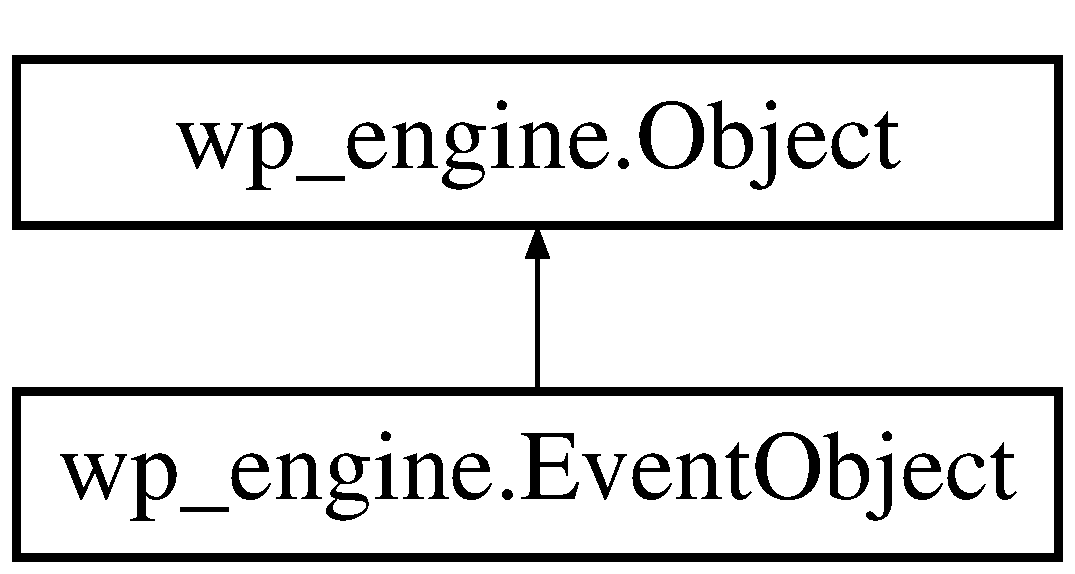
\includegraphics[height=2.000000cm]{classwp__engine_1_1_event_object}
\end{center}
\end{figure}
\subsection*{Public Member Functions}
\begin{DoxyCompactItemize}
\item 
\hyperlink{classwp__engine_1_1_event_object_a3e38dc176c260f8f642042a0e3754553}{Event\-Object} (float x, float y, Texture2\-D \hyperlink{classwp__engine_1_1_object_a5aebe29df25c51280d462cab63733c98}{texture})
\begin{DoxyCompactList}\small\item\em A constructor. \end{DoxyCompactList}\item 
\hypertarget{classwp__engine_1_1_event_object_a3abb3c66c76000c0d4d60ea55d024f13}{{\bfseries Event\-Object} (float x, float y, string asset\-Name)}\label{classwp__engine_1_1_event_object_a3abb3c66c76000c0d4d60ea55d024f13}

\item 
bool \hyperlink{classwp__engine_1_1_event_object_a32c433ab84ba60ca864f0dd9143fa339}{is\-Pressed} (Vector2 pressed\-Location)
\begin{DoxyCompactList}\small\item\em Returns true if parameter coordinates are inside the \hyperlink{classwp__engine_1_1_event_object}{Event\-Object}. \end{DoxyCompactList}\item 
\hypertarget{classwp__engine_1_1_event_object_a7a08fb371abceda36198f96b853fafea}{virtual void {\bfseries update} ()}\label{classwp__engine_1_1_event_object_a7a08fb371abceda36198f96b853fafea}

\end{DoxyCompactItemize}
\subsection*{Additional Inherited Members}


\subsection{Detailed Description}
A class of event handling objects. 

Part of the object partition.

Inherits \hyperlink{classwp__engine_1_1_object}{Object}. 

\subsection{Constructor \& Destructor Documentation}
\hypertarget{classwp__engine_1_1_event_object_a3e38dc176c260f8f642042a0e3754553}{\index{wp\-\_\-engine\-::\-Event\-Object@{wp\-\_\-engine\-::\-Event\-Object}!Event\-Object@{Event\-Object}}
\index{Event\-Object@{Event\-Object}!wp_engine::EventObject@{wp\-\_\-engine\-::\-Event\-Object}}
\subsubsection[{Event\-Object}]{\setlength{\rightskip}{0pt plus 5cm}wp\-\_\-engine.\-Event\-Object.\-Event\-Object (
\begin{DoxyParamCaption}
\item[{float}]{x, }
\item[{float}]{y, }
\item[{Texture2\-D}]{texture}
\end{DoxyParamCaption}
)\hspace{0.3cm}{\ttfamily [inline]}}}\label{classwp__engine_1_1_event_object_a3e38dc176c260f8f642042a0e3754553}


A constructor. 


\begin{DoxyParams}{Parameters}
{\em x} & object location (x-\/coordinate) \\
\hline
{\em y} & object location (y-\/coordinate) \\
\hline
{\em texture} & the texture of the object \\
\hline
\end{DoxyParams}


\subsection{Member Function Documentation}
\hypertarget{classwp__engine_1_1_event_object_a32c433ab84ba60ca864f0dd9143fa339}{\index{wp\-\_\-engine\-::\-Event\-Object@{wp\-\_\-engine\-::\-Event\-Object}!is\-Pressed@{is\-Pressed}}
\index{is\-Pressed@{is\-Pressed}!wp_engine::EventObject@{wp\-\_\-engine\-::\-Event\-Object}}
\subsubsection[{is\-Pressed}]{\setlength{\rightskip}{0pt plus 5cm}bool wp\-\_\-engine.\-Event\-Object.\-is\-Pressed (
\begin{DoxyParamCaption}
\item[{Vector2}]{pressed\-Location}
\end{DoxyParamCaption}
)\hspace{0.3cm}{\ttfamily [inline]}}}\label{classwp__engine_1_1_event_object_a32c433ab84ba60ca864f0dd9143fa339}


Returns true if parameter coordinates are inside the \hyperlink{classwp__engine_1_1_event_object}{Event\-Object}. 


\begin{DoxyParams}{Parameters}
{\em pressed\-Location} & the location which the user pressed (Vector2) \\
\hline
\end{DoxyParams}
\begin{DoxyReturn}{Returns}
boolean, true if parameter coordinates are inside the \hyperlink{classwp__engine_1_1_event_object}{Event\-Object} 
\end{DoxyReturn}


The documentation for this class was generated from the following file\-:\begin{DoxyCompactItemize}
\item 
Event\-Object.\-cs\end{DoxyCompactItemize}

\hypertarget{classwp__engine_1_1_help_state}{\section{wp\-\_\-engine.\-Help\-State Class Reference}
\label{classwp__engine_1_1_help_state}\index{wp\-\_\-engine.\-Help\-State@{wp\-\_\-engine.\-Help\-State}}
}


A class for help screens in games.  


Inheritance diagram for wp\-\_\-engine.\-Help\-State\-:\begin{figure}[H]
\begin{center}
\leavevmode
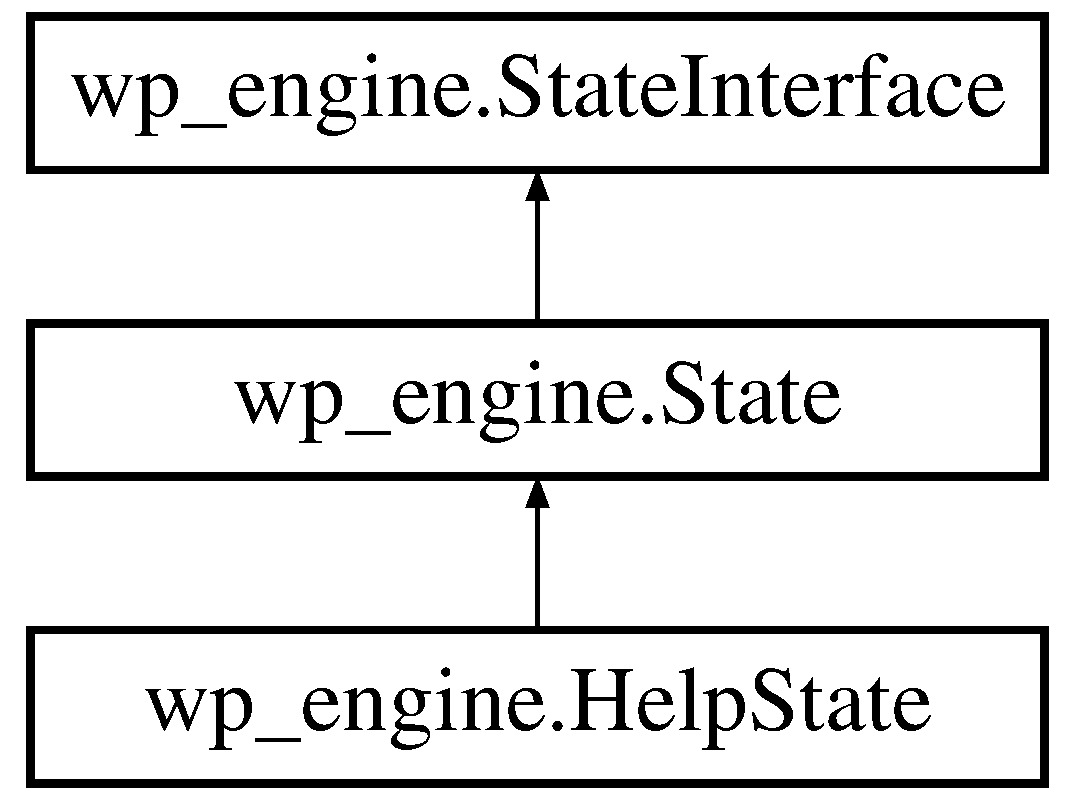
\includegraphics[height=3.000000cm]{classwp__engine_1_1_help_state}
\end{center}
\end{figure}
\subsection*{Public Member Functions}
\begin{DoxyCompactItemize}
\item 
\hyperlink{classwp__engine_1_1_help_state_a1916515cd4099c29f48f64474b6e5850}{Help\-State} (int screen\-Width, int screen\-Height)
\begin{DoxyCompactList}\small\item\em A constructor. \end{DoxyCompactList}\item 
\hypertarget{classwp__engine_1_1_help_state_ad929e3ae0212920f812240b50ed9379e}{override void {\bfseries init} ()}\label{classwp__engine_1_1_help_state_ad929e3ae0212920f812240b50ed9379e}

\item 
\hypertarget{classwp__engine_1_1_help_state_a7b235d6639cc38ef381fb693a72ec418}{override void {\bfseries update} (float elapsed)}\label{classwp__engine_1_1_help_state_a7b235d6639cc38ef381fb693a72ec418}

\item 
override void \hyperlink{classwp__engine_1_1_help_state_a2c671a3ef7985614c016bfb2881e3da2}{load\-Content} (Content\-Manager content\-Manager)
\begin{DoxyCompactList}\small\item\em The function loads the contents of the help screen. \end{DoxyCompactList}\end{DoxyCompactItemize}
\subsection*{Additional Inherited Members}


\subsection{Detailed Description}
A class for help screens in games. 

Part of the state partition.

Inherits \hyperlink{classwp__engine_1_1_state}{State}. 

\subsection{Constructor \& Destructor Documentation}
\hypertarget{classwp__engine_1_1_help_state_a1916515cd4099c29f48f64474b6e5850}{\index{wp\-\_\-engine\-::\-Help\-State@{wp\-\_\-engine\-::\-Help\-State}!Help\-State@{Help\-State}}
\index{Help\-State@{Help\-State}!wp_engine::HelpState@{wp\-\_\-engine\-::\-Help\-State}}
\subsubsection[{Help\-State}]{\setlength{\rightskip}{0pt plus 5cm}wp\-\_\-engine.\-Help\-State.\-Help\-State (
\begin{DoxyParamCaption}
\item[{int}]{screen\-Width, }
\item[{int}]{screen\-Height}
\end{DoxyParamCaption}
)\hspace{0.3cm}{\ttfamily [inline]}}}\label{classwp__engine_1_1_help_state_a1916515cd4099c29f48f64474b6e5850}


A constructor. 


\begin{DoxyParams}{Parameters}
{\em screen\-Width} & the width of the screen resolution \\
\hline
{\em screen\-Height} & the height of the screen resolution \\
\hline
\end{DoxyParams}


\subsection{Member Function Documentation}
\hypertarget{classwp__engine_1_1_help_state_a2c671a3ef7985614c016bfb2881e3da2}{\index{wp\-\_\-engine\-::\-Help\-State@{wp\-\_\-engine\-::\-Help\-State}!load\-Content@{load\-Content}}
\index{load\-Content@{load\-Content}!wp_engine::HelpState@{wp\-\_\-engine\-::\-Help\-State}}
\subsubsection[{load\-Content}]{\setlength{\rightskip}{0pt plus 5cm}override void wp\-\_\-engine.\-Help\-State.\-load\-Content (
\begin{DoxyParamCaption}
\item[{Content\-Manager}]{content\-Manager}
\end{DoxyParamCaption}
)\hspace{0.3cm}{\ttfamily [inline]}, {\ttfamily [virtual]}}}\label{classwp__engine_1_1_help_state_a2c671a3ef7985614c016bfb2881e3da2}


The function loads the contents of the help screen. 

Change this to your requirements. 
\begin{DoxyParams}{Parameters}
{\em content\-Manager} & the content manager for the game \\
\hline
\end{DoxyParams}


Reimplemented from \hyperlink{classwp__engine_1_1_state}{wp\-\_\-engine.\-State}.



The documentation for this class was generated from the following file\-:\begin{DoxyCompactItemize}
\item 
Help\-State.\-cs\end{DoxyCompactItemize}

\hypertarget{classwp__engine_1_1_live_object}{\section{wp\-\_\-engine.\-Live\-Object Class Reference}
\label{classwp__engine_1_1_live_object}\index{wp\-\_\-engine.\-Live\-Object@{wp\-\_\-engine.\-Live\-Object}}
}


A class for moving objects.  


Inheritance diagram for wp\-\_\-engine.\-Live\-Object\-:\begin{figure}[H]
\begin{center}
\leavevmode
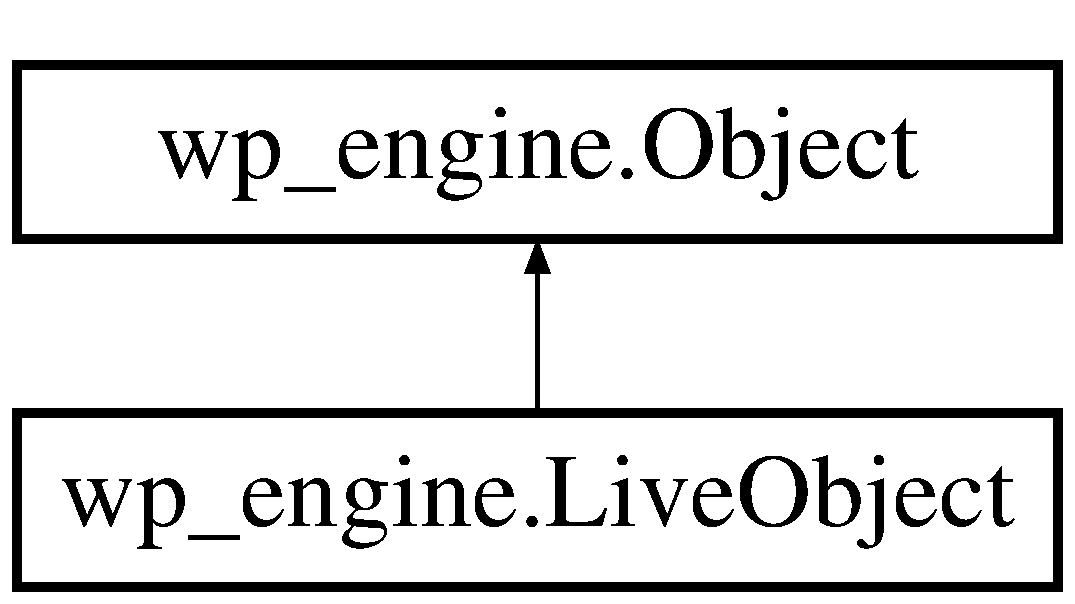
\includegraphics[height=2.000000cm]{classwp__engine_1_1_live_object}
\end{center}
\end{figure}
\subsection*{Public Member Functions}
\begin{DoxyCompactItemize}
\item 
\hyperlink{classwp__engine_1_1_live_object_a9df3b7ad35240319f760c7c02f24f453}{Live\-Object} (float x, float y, Texture2\-D \hyperlink{classwp__engine_1_1_object_a5aebe29df25c51280d462cab63733c98}{texture})
\begin{DoxyCompactList}\small\item\em A constructor. \end{DoxyCompactList}\item 
\hyperlink{classwp__engine_1_1_live_object_a4db779ac4b6c29bee18ad2f006d31c48}{Live\-Object} (float x, float y, Texture2\-D \hyperlink{classwp__engine_1_1_object_a5aebe29df25c51280d462cab63733c98}{texture}, Vector2 speed)
\begin{DoxyCompactList}\small\item\em A constructor. \end{DoxyCompactList}\item 
\hyperlink{classwp__engine_1_1_live_object_a98dd1f4bce092323ebe406f618099246}{Live\-Object} (float x, float y, Texture2\-D \hyperlink{classwp__engine_1_1_object_a5aebe29df25c51280d462cab63733c98}{texture}, Vector2 speed, Vector2 acceleration)
\begin{DoxyCompactList}\small\item\em A constructor. \end{DoxyCompactList}\item 
\hypertarget{classwp__engine_1_1_live_object_a0197e57f604dc1cb9e56440e193990e5}{{\bfseries Live\-Object} (float x, float y, string asset\-Name, Vector2 speed, Vector2 acceleration)}\label{classwp__engine_1_1_live_object_a0197e57f604dc1cb9e56440e193990e5}

\item 
virtual void \hyperlink{classwp__engine_1_1_live_object_af5db9ac2ecb0bc442ce6b43ffb1744b5}{update} ()
\begin{DoxyCompactList}\small\item\em Updates the object. \end{DoxyCompactList}\end{DoxyCompactItemize}
\subsection*{Protected Member Functions}
\begin{DoxyCompactItemize}
\item 
void \hyperlink{classwp__engine_1_1_live_object_a78341f24c3b41df7e8b1770beadce169}{move} ()
\begin{DoxyCompactList}\small\item\em Updates the speed and the location of the object. \end{DoxyCompactList}\end{DoxyCompactItemize}
\subsection*{Protected Attributes}
\begin{DoxyCompactItemize}
\item 
\hypertarget{classwp__engine_1_1_live_object_a754498ab3768aac3a96d378cf933ff24}{Vector2 {\bfseries acceleration}}\label{classwp__engine_1_1_live_object_a754498ab3768aac3a96d378cf933ff24}

\item 
\hypertarget{classwp__engine_1_1_live_object_a3d8e2a3dd8b63bcf09b1009f1533ce47}{Vector2 {\bfseries speed}}\label{classwp__engine_1_1_live_object_a3d8e2a3dd8b63bcf09b1009f1533ce47}

\end{DoxyCompactItemize}
\subsection*{Properties}
\begin{DoxyCompactItemize}
\item 
\hypertarget{classwp__engine_1_1_live_object_af077399d4235fc063fe8bc1f16250adf}{Vector2 \hyperlink{classwp__engine_1_1_live_object_af077399d4235fc063fe8bc1f16250adf}{Speed}\hspace{0.3cm}{\ttfamily  \mbox{[}get, set\mbox{]}}}\label{classwp__engine_1_1_live_object_af077399d4235fc063fe8bc1f16250adf}

\begin{DoxyCompactList}\small\item\em The speed of the object. \end{DoxyCompactList}\item 
\hypertarget{classwp__engine_1_1_live_object_a2d29e775cfabd3a3a0de7d50457722f6}{Vector2 \hyperlink{classwp__engine_1_1_live_object_a2d29e775cfabd3a3a0de7d50457722f6}{Acceleration}\hspace{0.3cm}{\ttfamily  \mbox{[}get, set\mbox{]}}}\label{classwp__engine_1_1_live_object_a2d29e775cfabd3a3a0de7d50457722f6}

\begin{DoxyCompactList}\small\item\em The acceleration of the object. \end{DoxyCompactList}\end{DoxyCompactItemize}
\subsection*{Additional Inherited Members}


\subsection{Detailed Description}
A class for moving objects. 

Part of the object partition.

Inherits \hyperlink{classwp__engine_1_1_object}{Object}. 

\subsection{Constructor \& Destructor Documentation}
\hypertarget{classwp__engine_1_1_live_object_a9df3b7ad35240319f760c7c02f24f453}{\index{wp\-\_\-engine\-::\-Live\-Object@{wp\-\_\-engine\-::\-Live\-Object}!Live\-Object@{Live\-Object}}
\index{Live\-Object@{Live\-Object}!wp_engine::LiveObject@{wp\-\_\-engine\-::\-Live\-Object}}
\subsubsection[{Live\-Object}]{\setlength{\rightskip}{0pt plus 5cm}wp\-\_\-engine.\-Live\-Object.\-Live\-Object (
\begin{DoxyParamCaption}
\item[{float}]{x, }
\item[{float}]{y, }
\item[{Texture2\-D}]{texture}
\end{DoxyParamCaption}
)\hspace{0.3cm}{\ttfamily [inline]}}}\label{classwp__engine_1_1_live_object_a9df3b7ad35240319f760c7c02f24f453}


A constructor. 

Sets initial speed and acceleration to zero. 
\begin{DoxyParams}{Parameters}
{\em x} & x-\/coordinate \\
\hline
{\em y} & y-\/coordinate \\
\hline
{\em texture} & the texture of the object \\
\hline
\end{DoxyParams}
\hypertarget{classwp__engine_1_1_live_object_a4db779ac4b6c29bee18ad2f006d31c48}{\index{wp\-\_\-engine\-::\-Live\-Object@{wp\-\_\-engine\-::\-Live\-Object}!Live\-Object@{Live\-Object}}
\index{Live\-Object@{Live\-Object}!wp_engine::LiveObject@{wp\-\_\-engine\-::\-Live\-Object}}
\subsubsection[{Live\-Object}]{\setlength{\rightskip}{0pt plus 5cm}wp\-\_\-engine.\-Live\-Object.\-Live\-Object (
\begin{DoxyParamCaption}
\item[{float}]{x, }
\item[{float}]{y, }
\item[{Texture2\-D}]{texture, }
\item[{Vector2}]{speed}
\end{DoxyParamCaption}
)\hspace{0.3cm}{\ttfamily [inline]}}}\label{classwp__engine_1_1_live_object_a4db779ac4b6c29bee18ad2f006d31c48}


A constructor. 

Sets initial acceleration to zero. 
\begin{DoxyParams}{Parameters}
{\em x} & x-\/coordinate \\
\hline
{\em y} & y-\/coordinate \\
\hline
{\em texture} & the texture of the object \\
\hline
{\em speed} & the initial speed of the object \\
\hline
\end{DoxyParams}
\hypertarget{classwp__engine_1_1_live_object_a98dd1f4bce092323ebe406f618099246}{\index{wp\-\_\-engine\-::\-Live\-Object@{wp\-\_\-engine\-::\-Live\-Object}!Live\-Object@{Live\-Object}}
\index{Live\-Object@{Live\-Object}!wp_engine::LiveObject@{wp\-\_\-engine\-::\-Live\-Object}}
\subsubsection[{Live\-Object}]{\setlength{\rightskip}{0pt plus 5cm}wp\-\_\-engine.\-Live\-Object.\-Live\-Object (
\begin{DoxyParamCaption}
\item[{float}]{x, }
\item[{float}]{y, }
\item[{Texture2\-D}]{texture, }
\item[{Vector2}]{speed, }
\item[{Vector2}]{acceleration}
\end{DoxyParamCaption}
)\hspace{0.3cm}{\ttfamily [inline]}}}\label{classwp__engine_1_1_live_object_a98dd1f4bce092323ebe406f618099246}


A constructor. 


\begin{DoxyParams}{Parameters}
{\em x} & x-\/coordinate \\
\hline
{\em y} & y-\/coordinate \\
\hline
{\em texture} & the texture of the object \\
\hline
{\em speed} & the initial speed of the object \\
\hline
{\em acceleration} & the initial acceleration of the object \\
\hline
\end{DoxyParams}


\subsection{Member Function Documentation}
\hypertarget{classwp__engine_1_1_live_object_a78341f24c3b41df7e8b1770beadce169}{\index{wp\-\_\-engine\-::\-Live\-Object@{wp\-\_\-engine\-::\-Live\-Object}!move@{move}}
\index{move@{move}!wp_engine::LiveObject@{wp\-\_\-engine\-::\-Live\-Object}}
\subsubsection[{move}]{\setlength{\rightskip}{0pt plus 5cm}void wp\-\_\-engine.\-Live\-Object.\-move (
\begin{DoxyParamCaption}
{}
\end{DoxyParamCaption}
)\hspace{0.3cm}{\ttfamily [inline]}, {\ttfamily [protected]}}}\label{classwp__engine_1_1_live_object_a78341f24c3b41df7e8b1770beadce169}


Updates the speed and the location of the object. 

Protected function. \hypertarget{classwp__engine_1_1_live_object_af5db9ac2ecb0bc442ce6b43ffb1744b5}{\index{wp\-\_\-engine\-::\-Live\-Object@{wp\-\_\-engine\-::\-Live\-Object}!update@{update}}
\index{update@{update}!wp_engine::LiveObject@{wp\-\_\-engine\-::\-Live\-Object}}
\subsubsection[{update}]{\setlength{\rightskip}{0pt plus 5cm}virtual void wp\-\_\-engine.\-Live\-Object.\-update (
\begin{DoxyParamCaption}
{}
\end{DoxyParamCaption}
)\hspace{0.3cm}{\ttfamily [inline]}, {\ttfamily [virtual]}}}\label{classwp__engine_1_1_live_object_af5db9ac2ecb0bc442ce6b43ffb1744b5}


Updates the object. 

Read\-: moves it. 

The documentation for this class was generated from the following file\-:\begin{DoxyCompactItemize}
\item 
Live\-Object.\-cs\end{DoxyCompactItemize}

\hypertarget{classwp__engine_1_1_menu_state}{\section{wp\-\_\-engine.\-Menu\-State Class Reference}
\label{classwp__engine_1_1_menu_state}\index{wp\-\_\-engine.\-Menu\-State@{wp\-\_\-engine.\-Menu\-State}}
}


A class for menu screen in a game.  


Inheritance diagram for wp\-\_\-engine.\-Menu\-State\-:\begin{figure}[H]
\begin{center}
\leavevmode
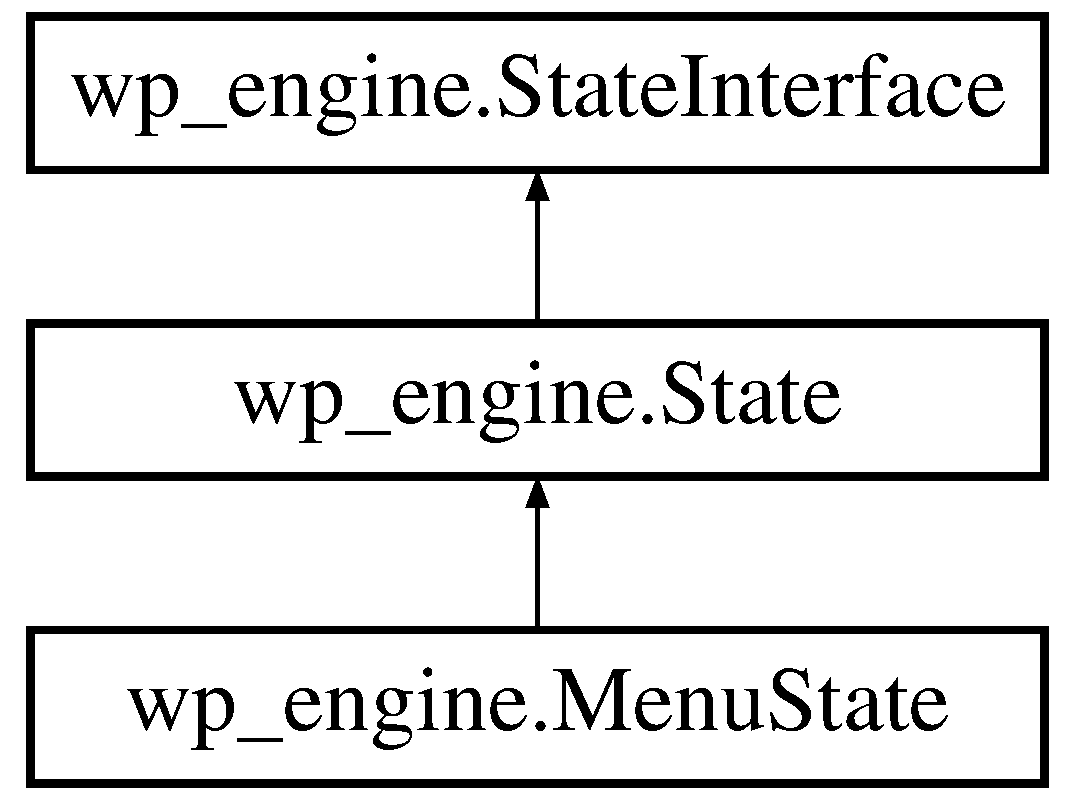
\includegraphics[height=3.000000cm]{classwp__engine_1_1_menu_state}
\end{center}
\end{figure}
\subsection*{Public Member Functions}
\begin{DoxyCompactItemize}
\item 
\hyperlink{classwp__engine_1_1_menu_state_a3d7c512948af3f51851890877d624df2}{Menu\-State} (int screen\-Width, int screen\-Height)
\begin{DoxyCompactList}\small\item\em A constructor. \end{DoxyCompactList}\item 
\hypertarget{classwp__engine_1_1_menu_state_ac621e5563b5e2332108f84945850ee1f}{override void {\bfseries init} ()}\label{classwp__engine_1_1_menu_state_ac621e5563b5e2332108f84945850ee1f}

\item 
\hypertarget{classwp__engine_1_1_menu_state_a39163feefdcb3ac49064c797ab112589}{override void {\bfseries update} (float elapsed)}\label{classwp__engine_1_1_menu_state_a39163feefdcb3ac49064c797ab112589}

\item 
override void \hyperlink{classwp__engine_1_1_menu_state_a3f2d385fae71f22cfa0dc432b4e90603}{load\-Content} (Content\-Manager content\-Manager)
\begin{DoxyCompactList}\small\item\em The function loads the contents of the help screen. \end{DoxyCompactList}\item 
override void \hyperlink{classwp__engine_1_1_menu_state_a59383f25558f805eca08fe6ac0ca70cd}{draw} (Sprite\-Batch sb)
\begin{DoxyCompactList}\small\item\em Draws the objects of the state. \end{DoxyCompactList}\end{DoxyCompactItemize}
\subsection*{Additional Inherited Members}


\subsection{Detailed Description}
A class for menu screen in a game. 

Part of the state partition.

Inherits \hyperlink{classwp__engine_1_1_state}{State}. 

\subsection{Constructor \& Destructor Documentation}
\hypertarget{classwp__engine_1_1_menu_state_a3d7c512948af3f51851890877d624df2}{\index{wp\-\_\-engine\-::\-Menu\-State@{wp\-\_\-engine\-::\-Menu\-State}!Menu\-State@{Menu\-State}}
\index{Menu\-State@{Menu\-State}!wp_engine::MenuState@{wp\-\_\-engine\-::\-Menu\-State}}
\subsubsection[{Menu\-State}]{\setlength{\rightskip}{0pt plus 5cm}wp\-\_\-engine.\-Menu\-State.\-Menu\-State (
\begin{DoxyParamCaption}
\item[{int}]{screen\-Width, }
\item[{int}]{screen\-Height}
\end{DoxyParamCaption}
)\hspace{0.3cm}{\ttfamily [inline]}}}\label{classwp__engine_1_1_menu_state_a3d7c512948af3f51851890877d624df2}


A constructor. 


\begin{DoxyParams}{Parameters}
{\em screen\-Width} & the width of the screen resolution \\
\hline
{\em screen\-Height} & the height of the screen resolution \\
\hline
\end{DoxyParams}


\subsection{Member Function Documentation}
\hypertarget{classwp__engine_1_1_menu_state_a59383f25558f805eca08fe6ac0ca70cd}{\index{wp\-\_\-engine\-::\-Menu\-State@{wp\-\_\-engine\-::\-Menu\-State}!draw@{draw}}
\index{draw@{draw}!wp_engine::MenuState@{wp\-\_\-engine\-::\-Menu\-State}}
\subsubsection[{draw}]{\setlength{\rightskip}{0pt plus 5cm}override void wp\-\_\-engine.\-Menu\-State.\-draw (
\begin{DoxyParamCaption}
\item[{Sprite\-Batch}]{sb}
\end{DoxyParamCaption}
)\hspace{0.3cm}{\ttfamily [inline]}, {\ttfamily [virtual]}}}\label{classwp__engine_1_1_menu_state_a59383f25558f805eca08fe6ac0ca70cd}


Draws the objects of the state. 


\begin{DoxyParams}{Parameters}
{\em sb} & the spritebatch of the game \\
\hline
\end{DoxyParams}


Reimplemented from \hyperlink{classwp__engine_1_1_state}{wp\-\_\-engine.\-State}.

\hypertarget{classwp__engine_1_1_menu_state_a3f2d385fae71f22cfa0dc432b4e90603}{\index{wp\-\_\-engine\-::\-Menu\-State@{wp\-\_\-engine\-::\-Menu\-State}!load\-Content@{load\-Content}}
\index{load\-Content@{load\-Content}!wp_engine::MenuState@{wp\-\_\-engine\-::\-Menu\-State}}
\subsubsection[{load\-Content}]{\setlength{\rightskip}{0pt plus 5cm}override void wp\-\_\-engine.\-Menu\-State.\-load\-Content (
\begin{DoxyParamCaption}
\item[{Content\-Manager}]{content\-Manager}
\end{DoxyParamCaption}
)\hspace{0.3cm}{\ttfamily [inline]}, {\ttfamily [virtual]}}}\label{classwp__engine_1_1_menu_state_a3f2d385fae71f22cfa0dc432b4e90603}


The function loads the contents of the help screen. 

Change this to your requirements. 
\begin{DoxyParams}{Parameters}
{\em content\-Manager} & the content manager for the game \\
\hline
\end{DoxyParams}


Reimplemented from \hyperlink{classwp__engine_1_1_state}{wp\-\_\-engine.\-State}.



The documentation for this class was generated from the following file\-:\begin{DoxyCompactItemize}
\item 
Menu\-State.\-cs\end{DoxyCompactItemize}

\hypertarget{classwp__engine_1_1_object}{\section{wp\-\_\-engine.\-Object Class Reference}
\label{classwp__engine_1_1_object}\index{wp\-\_\-engine.\-Object@{wp\-\_\-engine.\-Object}}
}


A class for graphical 2\-D objects.  


Inheritance diagram for wp\-\_\-engine.\-Object\-:\begin{figure}[H]
\begin{center}
\leavevmode
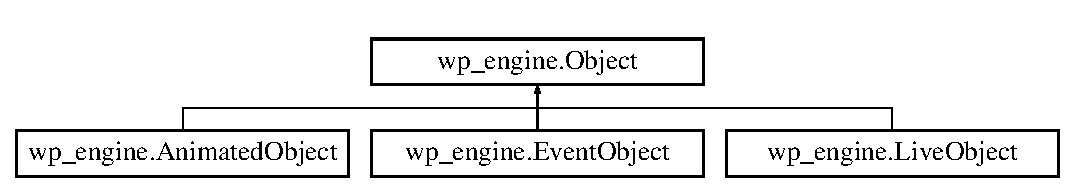
\includegraphics[height=2.000000cm]{classwp__engine_1_1_object}
\end{center}
\end{figure}
\subsection*{Public Member Functions}
\begin{DoxyCompactItemize}
\item 
\hyperlink{classwp__engine_1_1_object_a76308a1799d3e2a26da8cfbce0ab608e}{Object} (float x, float y, Texture2\-D \hyperlink{classwp__engine_1_1_object_a5aebe29df25c51280d462cab63733c98}{texture}, Layer layer)
\begin{DoxyCompactList}\small\item\em A constructor. \end{DoxyCompactList}\item 
\hyperlink{classwp__engine_1_1_object_ac41bd1d0ab2e99dd6de7e062bf2f5342}{Object} (Texture2\-D \hyperlink{classwp__engine_1_1_object_a5aebe29df25c51280d462cab63733c98}{texture}, Layer layer)
\begin{DoxyCompactList}\small\item\em A constructor. \end{DoxyCompactList}\item 
\hyperlink{classwp__engine_1_1_object_a0a364d6b59424f160dfbe81b60ecf138}{Object} (float x, float y, string texture\-Name, Layer layer)
\begin{DoxyCompactList}\small\item\em A constructor. \end{DoxyCompactList}\item 
void \hyperlink{classwp__engine_1_1_object_a7bec0bf1aadb96c3c4c570d0bc236738}{load\-Assets} (Content\-Manager content)
\begin{DoxyCompactList}\small\item\em Loads any unloaded assets. \end{DoxyCompactList}\item 
Vector2 \hyperlink{classwp__engine_1_1_object_a848ea6861e5132837e49a3171d1f885a}{get\-Center} ()
\begin{DoxyCompactList}\small\item\em Returns the location of the center of the object on the screen. \end{DoxyCompactList}\item 
void \hyperlink{classwp__engine_1_1_object_a8ae28b3c127cde23d39a2fec33dd910b}{set\-Location} (float x, float y)
\begin{DoxyCompactList}\small\item\em Used to set the location of the object. \end{DoxyCompactList}\item 
void \hyperlink{classwp__engine_1_1_object_ada86fb0b40d9232c839ce6d073023397}{draw} (Sprite\-Batch sb)
\begin{DoxyCompactList}\small\item\em Draws the object. \end{DoxyCompactList}\end{DoxyCompactItemize}
\subsection*{Static Public Member Functions}
\begin{DoxyCompactItemize}
\item 
static \hyperlink{classwp__engine_1_1_object}{Object} \hyperlink{classwp__engine_1_1_object_a0f9f6f59570251ad2003ea3bfa916730}{create\-Silent\-Object} (float x, float y, Texture2\-D \hyperlink{classwp__engine_1_1_object_a5aebe29df25c51280d462cab63733c98}{texture}, Layer layer)
\begin{DoxyCompactList}\small\item\em Returns a silent object. \end{DoxyCompactList}\item 
static \hyperlink{classwp__engine_1_1_object}{Object} \hyperlink{classwp__engine_1_1_object_a969b878e10457d6ef962db2c970e32a4}{create\-Silent\-Object} (float x, float y, string texture\-Name, Layer layer)
\begin{DoxyCompactList}\small\item\em Returns a silent object. \end{DoxyCompactList}\end{DoxyCompactItemize}
\subsection*{Protected Attributes}
\begin{DoxyCompactItemize}
\item 
\hypertarget{classwp__engine_1_1_object_a7329f71d51a64edeae4eecb5e7fccb27}{Vector2 {\bfseries location}}\label{classwp__engine_1_1_object_a7329f71d51a64edeae4eecb5e7fccb27}

\item 
\hypertarget{classwp__engine_1_1_object_a54782bfa242dd87f632d4c9829181746}{bool {\bfseries active}}\label{classwp__engine_1_1_object_a54782bfa242dd87f632d4c9829181746}

\item 
\hypertarget{classwp__engine_1_1_object_a26ff3315f04a4686d08ef3ee7e227227}{bool {\bfseries loaded}}\label{classwp__engine_1_1_object_a26ff3315f04a4686d08ef3ee7e227227}

\item 
\hypertarget{classwp__engine_1_1_object_aeca7deef83d80e53be3ec06ed7b42d00}{string {\bfseries asset\-Name}}\label{classwp__engine_1_1_object_aeca7deef83d80e53be3ec06ed7b42d00}

\item 
Texture2\-D \hyperlink{classwp__engine_1_1_object_a5aebe29df25c51280d462cab63733c98}{texture}
\begin{DoxyCompactList}\small\item\em The texture of the object. \end{DoxyCompactList}\item 
\hypertarget{classwp__engine_1_1_object_a55c63fadfe9ca3ae807a4f7b0fb222e0}{Layer {\bfseries layer}}\label{classwp__engine_1_1_object_a55c63fadfe9ca3ae807a4f7b0fb222e0}

\end{DoxyCompactItemize}
\subsection*{Properties}
\begin{DoxyCompactItemize}
\item 
\hypertarget{classwp__engine_1_1_object_a9b8c2e5191f6aa6971e82045e1dc4746}{bool \hyperlink{classwp__engine_1_1_object_a9b8c2e5191f6aa6971e82045e1dc4746}{Active}\hspace{0.3cm}{\ttfamily  \mbox{[}get, set\mbox{]}}}\label{classwp__engine_1_1_object_a9b8c2e5191f6aa6971e82045e1dc4746}

\begin{DoxyCompactList}\small\item\em A boolean variable that indicates whether or not the object should be updated and drawn. \end{DoxyCompactList}\item 
\hypertarget{classwp__engine_1_1_object_afb350e018ecade6b4869c617cf575d87}{Layer {\bfseries Draw\-Layer}\hspace{0.3cm}{\ttfamily  \mbox{[}get, set\mbox{]}}}\label{classwp__engine_1_1_object_afb350e018ecade6b4869c617cf575d87}

\item 
\hypertarget{classwp__engine_1_1_object_a04fc1210463e5919b256c3bb56640eff}{Vector2 \hyperlink{classwp__engine_1_1_object_a04fc1210463e5919b256c3bb56640eff}{Location}\hspace{0.3cm}{\ttfamily  \mbox{[}get, set\mbox{]}}}\label{classwp__engine_1_1_object_a04fc1210463e5919b256c3bb56640eff}

\begin{DoxyCompactList}\small\item\em Vector2 variable that stores the location of the object. \end{DoxyCompactList}\item 
\hypertarget{classwp__engine_1_1_object_a56bc69f58db1ef0e759c28a370328fab}{Vector2 {\bfseries Texture\-Size}\hspace{0.3cm}{\ttfamily  \mbox{[}get\mbox{]}}}\label{classwp__engine_1_1_object_a56bc69f58db1ef0e759c28a370328fab}

\end{DoxyCompactItemize}


\subsection{Detailed Description}
A class for graphical 2\-D objects. 

Part of the object partition.

The base class for all of the objects. 

\subsection{Constructor \& Destructor Documentation}
\hypertarget{classwp__engine_1_1_object_a76308a1799d3e2a26da8cfbce0ab608e}{\index{wp\-\_\-engine\-::\-Object@{wp\-\_\-engine\-::\-Object}!Object@{Object}}
\index{Object@{Object}!wp_engine::Object@{wp\-\_\-engine\-::\-Object}}
\subsubsection[{Object}]{\setlength{\rightskip}{0pt plus 5cm}wp\-\_\-engine.\-Object.\-Object (
\begin{DoxyParamCaption}
\item[{float}]{x, }
\item[{float}]{y, }
\item[{Texture2\-D}]{texture, }
\item[{Layer}]{layer}
\end{DoxyParamCaption}
)\hspace{0.3cm}{\ttfamily [inline]}}}\label{classwp__engine_1_1_object_a76308a1799d3e2a26da8cfbce0ab608e}


A constructor. 


\begin{DoxyParams}{Parameters}
{\em x} & object location (x-\/coordinate) \\
\hline
{\em y} & object location (y-\/coordinate) \\
\hline
{\em texture} & the picture which the object represents \\
\hline
\end{DoxyParams}
\hypertarget{classwp__engine_1_1_object_ac41bd1d0ab2e99dd6de7e062bf2f5342}{\index{wp\-\_\-engine\-::\-Object@{wp\-\_\-engine\-::\-Object}!Object@{Object}}
\index{Object@{Object}!wp_engine::Object@{wp\-\_\-engine\-::\-Object}}
\subsubsection[{Object}]{\setlength{\rightskip}{0pt plus 5cm}wp\-\_\-engine.\-Object.\-Object (
\begin{DoxyParamCaption}
\item[{Texture2\-D}]{texture, }
\item[{Layer}]{layer}
\end{DoxyParamCaption}
)\hspace{0.3cm}{\ttfamily [inline]}}}\label{classwp__engine_1_1_object_ac41bd1d0ab2e99dd6de7e062bf2f5342}


A constructor. 

Sets the object location to (0, 0). 
\begin{DoxyParams}{Parameters}
{\em texture} & the picture which the object represents \\
\hline
\end{DoxyParams}
\hypertarget{classwp__engine_1_1_object_a0a364d6b59424f160dfbe81b60ecf138}{\index{wp\-\_\-engine\-::\-Object@{wp\-\_\-engine\-::\-Object}!Object@{Object}}
\index{Object@{Object}!wp_engine::Object@{wp\-\_\-engine\-::\-Object}}
\subsubsection[{Object}]{\setlength{\rightskip}{0pt plus 5cm}wp\-\_\-engine.\-Object.\-Object (
\begin{DoxyParamCaption}
\item[{float}]{x, }
\item[{float}]{y, }
\item[{string}]{texture\-Name, }
\item[{Layer}]{layer}
\end{DoxyParamCaption}
)\hspace{0.3cm}{\ttfamily [inline]}}}\label{classwp__engine_1_1_object_a0a364d6b59424f160dfbe81b60ecf138}


A constructor. 

Creates an object without without having to load the texture (yet). 
\begin{DoxyParams}{Parameters}
{\em x} & object location (x-\/coordinate) \\
\hline
{\em y} & object location (y-\/coordinate) \\
\hline
{\em texture\-Name} & the name of the picture which the object represents \\
\hline
\end{DoxyParams}


\subsection{Member Function Documentation}
\hypertarget{classwp__engine_1_1_object_a0f9f6f59570251ad2003ea3bfa916730}{\index{wp\-\_\-engine\-::\-Object@{wp\-\_\-engine\-::\-Object}!create\-Silent\-Object@{create\-Silent\-Object}}
\index{create\-Silent\-Object@{create\-Silent\-Object}!wp_engine::Object@{wp\-\_\-engine\-::\-Object}}
\subsubsection[{create\-Silent\-Object}]{\setlength{\rightskip}{0pt plus 5cm}static {\bf Object} wp\-\_\-engine.\-Object.\-create\-Silent\-Object (
\begin{DoxyParamCaption}
\item[{float}]{x, }
\item[{float}]{y, }
\item[{Texture2\-D}]{texture, }
\item[{Layer}]{layer}
\end{DoxyParamCaption}
)\hspace{0.3cm}{\ttfamily [inline]}, {\ttfamily [static]}}}\label{classwp__engine_1_1_object_a0f9f6f59570251ad2003ea3bfa916730}


Returns a silent object. 

It won't be updated or drawn unless specified otherwise.


\begin{DoxyParams}{Parameters}
{\em x} & object location (x-\/coordinate) \\
\hline
{\em y} & object location (y-\/coordinate) \\
\hline
{\em texture} & the picture which the object represents \\
\hline
\end{DoxyParams}
\hypertarget{classwp__engine_1_1_object_a969b878e10457d6ef962db2c970e32a4}{\index{wp\-\_\-engine\-::\-Object@{wp\-\_\-engine\-::\-Object}!create\-Silent\-Object@{create\-Silent\-Object}}
\index{create\-Silent\-Object@{create\-Silent\-Object}!wp_engine::Object@{wp\-\_\-engine\-::\-Object}}
\subsubsection[{create\-Silent\-Object}]{\setlength{\rightskip}{0pt plus 5cm}static {\bf Object} wp\-\_\-engine.\-Object.\-create\-Silent\-Object (
\begin{DoxyParamCaption}
\item[{float}]{x, }
\item[{float}]{y, }
\item[{string}]{texture\-Name, }
\item[{Layer}]{layer}
\end{DoxyParamCaption}
)\hspace{0.3cm}{\ttfamily [inline]}, {\ttfamily [static]}}}\label{classwp__engine_1_1_object_a969b878e10457d6ef962db2c970e32a4}


Returns a silent object. 

It won't be updated or drawn unless specified otherwise.


\begin{DoxyParams}{Parameters}
{\em x} & object location (x-\/coordinate) \\
\hline
{\em y} & object location (y-\/coordinate) \\
\hline
{\em texture\-Name} & the name of the picture which the object represents \\
\hline
\end{DoxyParams}
\hypertarget{classwp__engine_1_1_object_ada86fb0b40d9232c839ce6d073023397}{\index{wp\-\_\-engine\-::\-Object@{wp\-\_\-engine\-::\-Object}!draw@{draw}}
\index{draw@{draw}!wp_engine::Object@{wp\-\_\-engine\-::\-Object}}
\subsubsection[{draw}]{\setlength{\rightskip}{0pt plus 5cm}void wp\-\_\-engine.\-Object.\-draw (
\begin{DoxyParamCaption}
\item[{Sprite\-Batch}]{sb}
\end{DoxyParamCaption}
)\hspace{0.3cm}{\ttfamily [inline]}}}\label{classwp__engine_1_1_object_ada86fb0b40d9232c839ce6d073023397}


Draws the object. 


\begin{DoxyParams}{Parameters}
{\em sb} & the spritebatch of the game \\
\hline
\end{DoxyParams}
\hypertarget{classwp__engine_1_1_object_a848ea6861e5132837e49a3171d1f885a}{\index{wp\-\_\-engine\-::\-Object@{wp\-\_\-engine\-::\-Object}!get\-Center@{get\-Center}}
\index{get\-Center@{get\-Center}!wp_engine::Object@{wp\-\_\-engine\-::\-Object}}
\subsubsection[{get\-Center}]{\setlength{\rightskip}{0pt plus 5cm}Vector2 wp\-\_\-engine.\-Object.\-get\-Center (
\begin{DoxyParamCaption}
{}
\end{DoxyParamCaption}
)\hspace{0.3cm}{\ttfamily [inline]}}}\label{classwp__engine_1_1_object_a848ea6861e5132837e49a3171d1f885a}


Returns the location of the center of the object on the screen. 

\begin{DoxyReturn}{Returns}
the coordinates of the object's center (Vector2) 
\end{DoxyReturn}
\hypertarget{classwp__engine_1_1_object_a7bec0bf1aadb96c3c4c570d0bc236738}{\index{wp\-\_\-engine\-::\-Object@{wp\-\_\-engine\-::\-Object}!load\-Assets@{load\-Assets}}
\index{load\-Assets@{load\-Assets}!wp_engine::Object@{wp\-\_\-engine\-::\-Object}}
\subsubsection[{load\-Assets}]{\setlength{\rightskip}{0pt plus 5cm}void wp\-\_\-engine.\-Object.\-load\-Assets (
\begin{DoxyParamCaption}
\item[{Content\-Manager}]{content}
\end{DoxyParamCaption}
)\hspace{0.3cm}{\ttfamily [inline]}}}\label{classwp__engine_1_1_object_a7bec0bf1aadb96c3c4c570d0bc236738}


Loads any unloaded assets. 


\begin{DoxyParams}{Parameters}
{\em content} & the Content\-Manager of the game \\
\hline
\end{DoxyParams}
\hypertarget{classwp__engine_1_1_object_a8ae28b3c127cde23d39a2fec33dd910b}{\index{wp\-\_\-engine\-::\-Object@{wp\-\_\-engine\-::\-Object}!set\-Location@{set\-Location}}
\index{set\-Location@{set\-Location}!wp_engine::Object@{wp\-\_\-engine\-::\-Object}}
\subsubsection[{set\-Location}]{\setlength{\rightskip}{0pt plus 5cm}void wp\-\_\-engine.\-Object.\-set\-Location (
\begin{DoxyParamCaption}
\item[{float}]{x, }
\item[{float}]{y}
\end{DoxyParamCaption}
)\hspace{0.3cm}{\ttfamily [inline]}}}\label{classwp__engine_1_1_object_a8ae28b3c127cde23d39a2fec33dd910b}


Used to set the location of the object. 


\begin{DoxyParams}{Parameters}
{\em x} & x-\/coordinate \\
\hline
{\em y} & y-\/coordinate \\
\hline
\end{DoxyParams}


\subsection{Member Data Documentation}
\hypertarget{classwp__engine_1_1_object_a5aebe29df25c51280d462cab63733c98}{\index{wp\-\_\-engine\-::\-Object@{wp\-\_\-engine\-::\-Object}!texture@{texture}}
\index{texture@{texture}!wp_engine::Object@{wp\-\_\-engine\-::\-Object}}
\subsubsection[{texture}]{\setlength{\rightskip}{0pt plus 5cm}Texture2\-D wp\-\_\-engine.\-Object.\-texture\hspace{0.3cm}{\ttfamily [protected]}}}\label{classwp__engine_1_1_object_a5aebe29df25c51280d462cab63733c98}


The texture of the object. 



The documentation for this class was generated from the following file\-:\begin{DoxyCompactItemize}
\item 
Object.\-cs\end{DoxyCompactItemize}

\hypertarget{classwp__engine_1_1_slide_show}{\section{wp\-\_\-engine.\-Slide\-Show Class Reference}
\label{classwp__engine_1_1_slide_show}\index{wp\-\_\-engine.\-Slide\-Show@{wp\-\_\-engine.\-Slide\-Show}}
}


A class for multiple animation\-: a slideshow.  


\subsection*{Public Member Functions}
\begin{DoxyCompactItemize}
\item 
\hyperlink{classwp__engine_1_1_slide_show_afc5fccb2413a851f53ce4fef36c7e265}{Slide\-Show} ()
\begin{DoxyCompactList}\small\item\em A constructor. \end{DoxyCompactList}\item 
void \hyperlink{classwp__engine_1_1_slide_show_a0dd7f71b3beabc241f1b537bb3e7e5e7}{add\-Animated\-Object} (\hyperlink{classwp__engine_1_1_animated_object}{Animated\-Object} animated\-Object)
\begin{DoxyCompactList}\small\item\em Adds an animated object (animation). \end{DoxyCompactList}\item 
void \hyperlink{classwp__engine_1_1_slide_show_a77b840d961b07ca4c123ecfb1179f8f2}{update} (float elapsed)
\begin{DoxyCompactList}\small\item\em Updates the current animation. \end{DoxyCompactList}\item 
\hypertarget{classwp__engine_1_1_slide_show_a030f369d8cd2de1fdbe1198e18f77bd2}{void \hyperlink{classwp__engine_1_1_slide_show_a030f369d8cd2de1fdbe1198e18f77bd2}{next} ()}\label{classwp__engine_1_1_slide_show_a030f369d8cd2de1fdbe1198e18f77bd2}

\begin{DoxyCompactList}\small\item\em Activates the next animation in the slideshow. \end{DoxyCompactList}\item 
void \hyperlink{classwp__engine_1_1_slide_show_a4015703b2d7d1eb24e48059823e6cbc2}{auto\-Update} (float elapsed)
\begin{DoxyCompactList}\small\item\em Updates the slideshow and changes the animation automatically once the animation has been shown completely. \end{DoxyCompactList}\item 
void \hyperlink{classwp__engine_1_1_slide_show_ae9e09fb9ebac00528557f756de8ce0e4}{draw} (Sprite\-Batch sb)
\begin{DoxyCompactList}\small\item\em Draws the current frame of the current animation. \end{DoxyCompactList}\item 
void \hyperlink{classwp__engine_1_1_slide_show_abca02602546c159a475dc1f31836d47f}{stop} ()
\begin{DoxyCompactList}\small\item\em Stops the slideshow. \end{DoxyCompactList}\item 
void \hyperlink{classwp__engine_1_1_slide_show_a6b9e6fa9b5a79b1ed9b5097f1141ed56}{resume} ()
\begin{DoxyCompactList}\small\item\em Resumes the slideshow. \end{DoxyCompactList}\end{DoxyCompactItemize}


\subsection{Detailed Description}
A class for multiple animation\-: a slideshow. 

The idea is that a slideshow contains multiple animations and the animation that is displayed can be changed by an event.

Part of the animation partition. 

\subsection{Constructor \& Destructor Documentation}
\hypertarget{classwp__engine_1_1_slide_show_afc5fccb2413a851f53ce4fef36c7e265}{\index{wp\-\_\-engine\-::\-Slide\-Show@{wp\-\_\-engine\-::\-Slide\-Show}!Slide\-Show@{Slide\-Show}}
\index{Slide\-Show@{Slide\-Show}!wp_engine::SlideShow@{wp\-\_\-engine\-::\-Slide\-Show}}
\subsubsection[{Slide\-Show}]{\setlength{\rightskip}{0pt plus 5cm}wp\-\_\-engine.\-Slide\-Show.\-Slide\-Show (
\begin{DoxyParamCaption}
{}
\end{DoxyParamCaption}
)\hspace{0.3cm}{\ttfamily [inline]}}}\label{classwp__engine_1_1_slide_show_afc5fccb2413a851f53ce4fef36c7e265}


A constructor. 

Sets the variables to default values. 

\subsection{Member Function Documentation}
\hypertarget{classwp__engine_1_1_slide_show_a0dd7f71b3beabc241f1b537bb3e7e5e7}{\index{wp\-\_\-engine\-::\-Slide\-Show@{wp\-\_\-engine\-::\-Slide\-Show}!add\-Animated\-Object@{add\-Animated\-Object}}
\index{add\-Animated\-Object@{add\-Animated\-Object}!wp_engine::SlideShow@{wp\-\_\-engine\-::\-Slide\-Show}}
\subsubsection[{add\-Animated\-Object}]{\setlength{\rightskip}{0pt plus 5cm}void wp\-\_\-engine.\-Slide\-Show.\-add\-Animated\-Object (
\begin{DoxyParamCaption}
\item[{{\bf Animated\-Object}}]{animated\-Object}
\end{DoxyParamCaption}
)\hspace{0.3cm}{\ttfamily [inline]}}}\label{classwp__engine_1_1_slide_show_a0dd7f71b3beabc241f1b537bb3e7e5e7}


Adds an animated object (animation). 


\begin{DoxyParams}{Parameters}
{\em animated\-Object} & the \hyperlink{classwp__engine_1_1_animated_object}{Animated\-Object} containing the animation you wish to add \\
\hline
\end{DoxyParams}
\hypertarget{classwp__engine_1_1_slide_show_a4015703b2d7d1eb24e48059823e6cbc2}{\index{wp\-\_\-engine\-::\-Slide\-Show@{wp\-\_\-engine\-::\-Slide\-Show}!auto\-Update@{auto\-Update}}
\index{auto\-Update@{auto\-Update}!wp_engine::SlideShow@{wp\-\_\-engine\-::\-Slide\-Show}}
\subsubsection[{auto\-Update}]{\setlength{\rightskip}{0pt plus 5cm}void wp\-\_\-engine.\-Slide\-Show.\-auto\-Update (
\begin{DoxyParamCaption}
\item[{float}]{elapsed}
\end{DoxyParamCaption}
)\hspace{0.3cm}{\ttfamily [inline]}}}\label{classwp__engine_1_1_slide_show_a4015703b2d7d1eb24e48059823e6cbc2}


Updates the slideshow and changes the animation automatically once the animation has been shown completely. 


\begin{DoxyParams}{Parameters}
{\em elapsed} & elapsed time \\
\hline
\end{DoxyParams}
\hypertarget{classwp__engine_1_1_slide_show_ae9e09fb9ebac00528557f756de8ce0e4}{\index{wp\-\_\-engine\-::\-Slide\-Show@{wp\-\_\-engine\-::\-Slide\-Show}!draw@{draw}}
\index{draw@{draw}!wp_engine::SlideShow@{wp\-\_\-engine\-::\-Slide\-Show}}
\subsubsection[{draw}]{\setlength{\rightskip}{0pt plus 5cm}void wp\-\_\-engine.\-Slide\-Show.\-draw (
\begin{DoxyParamCaption}
\item[{Sprite\-Batch}]{sb}
\end{DoxyParamCaption}
)\hspace{0.3cm}{\ttfamily [inline]}}}\label{classwp__engine_1_1_slide_show_ae9e09fb9ebac00528557f756de8ce0e4}


Draws the current frame of the current animation. 


\begin{DoxyParams}{Parameters}
{\em sb} & the spritebatch of the game \\
\hline
\end{DoxyParams}
\hypertarget{classwp__engine_1_1_slide_show_a6b9e6fa9b5a79b1ed9b5097f1141ed56}{\index{wp\-\_\-engine\-::\-Slide\-Show@{wp\-\_\-engine\-::\-Slide\-Show}!resume@{resume}}
\index{resume@{resume}!wp_engine::SlideShow@{wp\-\_\-engine\-::\-Slide\-Show}}
\subsubsection[{resume}]{\setlength{\rightskip}{0pt plus 5cm}void wp\-\_\-engine.\-Slide\-Show.\-resume (
\begin{DoxyParamCaption}
{}
\end{DoxyParamCaption}
)\hspace{0.3cm}{\ttfamily [inline]}}}\label{classwp__engine_1_1_slide_show_a6b9e6fa9b5a79b1ed9b5097f1141ed56}


Resumes the slideshow. 

Resumes \hyperlink{classwp__engine_1_1_slide_show_a4015703b2d7d1eb24e48059823e6cbc2}{auto\-Update()}, and the current animation. Enables \hyperlink{classwp__engine_1_1_slide_show_a030f369d8cd2de1fdbe1198e18f77bd2}{next()} function. \hypertarget{classwp__engine_1_1_slide_show_abca02602546c159a475dc1f31836d47f}{\index{wp\-\_\-engine\-::\-Slide\-Show@{wp\-\_\-engine\-::\-Slide\-Show}!stop@{stop}}
\index{stop@{stop}!wp_engine::SlideShow@{wp\-\_\-engine\-::\-Slide\-Show}}
\subsubsection[{stop}]{\setlength{\rightskip}{0pt plus 5cm}void wp\-\_\-engine.\-Slide\-Show.\-stop (
\begin{DoxyParamCaption}
{}
\end{DoxyParamCaption}
)\hspace{0.3cm}{\ttfamily [inline]}}}\label{classwp__engine_1_1_slide_show_abca02602546c159a475dc1f31836d47f}


Stops the slideshow. 

Stops \hyperlink{classwp__engine_1_1_slide_show_a4015703b2d7d1eb24e48059823e6cbc2}{auto\-Update()}, and the current animation. Disables \hyperlink{classwp__engine_1_1_slide_show_a030f369d8cd2de1fdbe1198e18f77bd2}{next()} function. \hypertarget{classwp__engine_1_1_slide_show_a77b840d961b07ca4c123ecfb1179f8f2}{\index{wp\-\_\-engine\-::\-Slide\-Show@{wp\-\_\-engine\-::\-Slide\-Show}!update@{update}}
\index{update@{update}!wp_engine::SlideShow@{wp\-\_\-engine\-::\-Slide\-Show}}
\subsubsection[{update}]{\setlength{\rightskip}{0pt plus 5cm}void wp\-\_\-engine.\-Slide\-Show.\-update (
\begin{DoxyParamCaption}
\item[{float}]{elapsed}
\end{DoxyParamCaption}
)\hspace{0.3cm}{\ttfamily [inline]}}}\label{classwp__engine_1_1_slide_show_a77b840d961b07ca4c123ecfb1179f8f2}


Updates the current animation. 


\begin{DoxyParams}{Parameters}
{\em elapsed} & elapsed time \\
\hline
\end{DoxyParams}


The documentation for this class was generated from the following file\-:\begin{DoxyCompactItemize}
\item 
Slide\-Show.\-cs\end{DoxyCompactItemize}

\hypertarget{classwp__engine_1_1_state}{\section{wp\-\_\-engine.\-State Class Reference}
\label{classwp__engine_1_1_state}\index{wp\-\_\-engine.\-State@{wp\-\_\-engine.\-State}}
}


The base class for all of the game states.  


Inheritance diagram for wp\-\_\-engine.\-State\-:\begin{figure}[H]
\begin{center}
\leavevmode
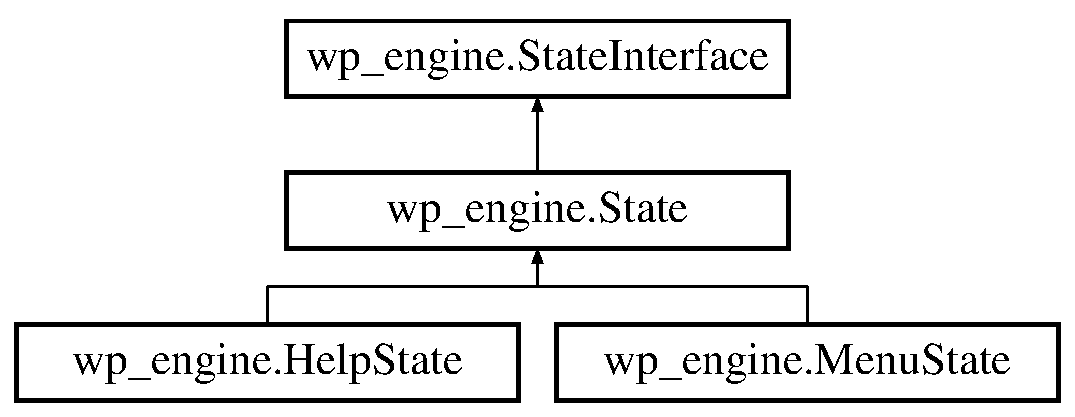
\includegraphics[height=3.000000cm]{classwp__engine_1_1_state}
\end{center}
\end{figure}
\subsection*{Public Member Functions}
\begin{DoxyCompactItemize}
\item 
\hypertarget{classwp__engine_1_1_state_a6751338962e6da93c8b9afc859df9762}{delegate void {\bfseries method} ()}\label{classwp__engine_1_1_state_a6751338962e6da93c8b9afc859df9762}

\item 
\hyperlink{classwp__engine_1_1_state_a7b0929ccee00bfae0591b4f2d5bb57a7}{State} (int screen\-Width, int screen\-Height)
\begin{DoxyCompactList}\small\item\em A constructor. \end{DoxyCompactList}\item 
\hypertarget{classwp__engine_1_1_state_a3aac3b299c00af7ba2c91b65b873dcfc}{virtual void {\bfseries init} ()}\label{classwp__engine_1_1_state_a3aac3b299c00af7ba2c91b65b873dcfc}

\item 
\hypertarget{classwp__engine_1_1_state_a13c88b5362a424a22b8b66deae2695d5}{virtual void {\bfseries update} (float elapsed\-Time)}\label{classwp__engine_1_1_state_a13c88b5362a424a22b8b66deae2695d5}

\item 
\hypertarget{classwp__engine_1_1_state_aacb9e5cd0e6eebe165029d8410c04855}{virtual void {\bfseries load\-Content} (Content\-Manager content\-Manager)}\label{classwp__engine_1_1_state_aacb9e5cd0e6eebe165029d8410c04855}

\item 
\hypertarget{classwp__engine_1_1_state_a54cd59a5cefff596966c18d4b66f942b}{virtual void {\bfseries draw} (Sprite\-Batch sb)}\label{classwp__engine_1_1_state_a54cd59a5cefff596966c18d4b66f942b}

\item 
virtual \hyperlink{namespacewp__engine_aae123481cdcc6dc4c4474c1b0b62b152}{state\-Identifier} \hyperlink{classwp__engine_1_1_state_a9373a9a657364683fa648f655bc323a7}{requests} (\hyperlink{classwp__engine_1_1_event}{Event} recent\-Event)
\begin{DoxyCompactList}\small\item\em Reacts to events. \end{DoxyCompactList}\item 
\hypertarget{classwp__engine_1_1_state_a9b58df33e71d1f9d8fbe3b6521ce9b93}{void {\bfseries add\-Bitmap} (float x, float y, string texture\-Name, Layer layer)}\label{classwp__engine_1_1_state_a9b58df33e71d1f9d8fbe3b6521ce9b93}

\item 
\hypertarget{classwp__engine_1_1_state_ade2cc3e6fe0619d9727511599abebedf}{void {\bfseries add\-Silent\-Bitmap} (float x, float y, string texture\-Name, Layer layer)}\label{classwp__engine_1_1_state_ade2cc3e6fe0619d9727511599abebedf}

\item 
\hypertarget{classwp__engine_1_1_state_a6fc3e1da80ea7ca94223c0cdff25bc05}{void {\bfseries add\-State\-Button} (\hyperlink{namespacewp__engine_aae123481cdcc6dc4c4474c1b0b62b152}{state\-Identifier} target\-State, float x, float y, string texture\-Name)}\label{classwp__engine_1_1_state_a6fc3e1da80ea7ca94223c0cdff25bc05}

\item 
\hypertarget{classwp__engine_1_1_state_a437af65520e3d7eb5c3e64221a4019f9}{void {\bfseries add\-Sound\-Effect} (Content\-Manager content, string file\-Name)}\label{classwp__engine_1_1_state_a437af65520e3d7eb5c3e64221a4019f9}

\end{DoxyCompactItemize}
\subsection*{Protected Attributes}
\begin{DoxyCompactItemize}
\item 
\hypertarget{classwp__engine_1_1_state_a73bf7aa957cff5e5e91b7015daa2894f}{Vector2 \hyperlink{classwp__engine_1_1_state_a73bf7aa957cff5e5e91b7015daa2894f}{resolution}}\label{classwp__engine_1_1_state_a73bf7aa957cff5e5e91b7015daa2894f}

\begin{DoxyCompactList}\small\item\em The resolution of the screen. \end{DoxyCompactList}\item 
\hypertarget{classwp__engine_1_1_state_a53ed789963fc0d6863ecbbe34a902d5e}{List$<$ \hyperlink{classwp__engine_1_1_object}{Object} $>$ \hyperlink{classwp__engine_1_1_state_a53ed789963fc0d6863ecbbe34a902d5e}{bitmaps}}\label{classwp__engine_1_1_state_a53ed789963fc0d6863ecbbe34a902d5e}

\begin{DoxyCompactList}\small\item\em Contains all of the object that act as simple pictures. \end{DoxyCompactList}\item 
\hypertarget{classwp__engine_1_1_state_abcdac647febd7fa9d599e679c3367848}{List$<$ \hyperlink{classwp__engine_1_1_live_object}{Live\-Object} $>$ \hyperlink{classwp__engine_1_1_state_abcdac647febd7fa9d599e679c3367848}{live\-Objects}}\label{classwp__engine_1_1_state_abcdac647febd7fa9d599e679c3367848}

\begin{DoxyCompactList}\small\item\em Contains moving objects. \end{DoxyCompactList}\item 
\hypertarget{classwp__engine_1_1_state_a19e966030739c40f4c8f6e3a1476f02e}{Dictionary$<$ method, \hyperlink{classwp__engine_1_1_event_object}{Event\-Object} $>$ \hyperlink{classwp__engine_1_1_state_a19e966030739c40f4c8f6e3a1476f02e}{method\-Buttons}}\label{classwp__engine_1_1_state_a19e966030739c40f4c8f6e3a1476f02e}

\begin{DoxyCompactList}\small\item\em Contains buttons that trigger a method. \end{DoxyCompactList}\item 
\hypertarget{classwp__engine_1_1_state_a4c5480cd2be3f954d88417d24aee6029}{Dictionary$<$ \hyperlink{namespacewp__engine_aae123481cdcc6dc4c4474c1b0b62b152}{state\-Identifier}, \\*
\hyperlink{classwp__engine_1_1_event_object}{Event\-Object} $>$ \hyperlink{classwp__engine_1_1_state_a4c5480cd2be3f954d88417d24aee6029}{state\-Buttons}}\label{classwp__engine_1_1_state_a4c5480cd2be3f954d88417d24aee6029}

\begin{DoxyCompactList}\small\item\em Constains buttons that trigger a state transition. \end{DoxyCompactList}\item 
\hyperlink{classwp__engine_1_1_audio_handler}{Audio\-Handler} \hyperlink{classwp__engine_1_1_state_a858efbade97385348071d3fba522f712}{audio\-Handler}
\begin{DoxyCompactList}\small\item\em The \hyperlink{classwp__engine_1_1_audio_handler}{Audio\-Handler} for the state. \end{DoxyCompactList}\end{DoxyCompactItemize}


\subsection{Detailed Description}
The base class for all of the game states. 

(ie. \hyperlink{classwp__engine_1_1_help_state}{Help\-State}, \hyperlink{classwp__engine_1_1_menu_state}{Menu\-State}) Part of the state Partition.

Implements \hyperlink{interfacewp__engine_1_1_state_interface}{State\-Interface}. 

\subsection{Constructor \& Destructor Documentation}
\hypertarget{classwp__engine_1_1_state_a7b0929ccee00bfae0591b4f2d5bb57a7}{\index{wp\-\_\-engine\-::\-State@{wp\-\_\-engine\-::\-State}!State@{State}}
\index{State@{State}!wp_engine::State@{wp\-\_\-engine\-::\-State}}
\subsubsection[{State}]{\setlength{\rightskip}{0pt plus 5cm}wp\-\_\-engine.\-State.\-State (
\begin{DoxyParamCaption}
\item[{int}]{screen\-Width, }
\item[{int}]{screen\-Height}
\end{DoxyParamCaption}
)\hspace{0.3cm}{\ttfamily [inline]}}}\label{classwp__engine_1_1_state_a7b0929ccee00bfae0591b4f2d5bb57a7}


A constructor. 


\begin{DoxyParams}{Parameters}
{\em screen\-Width} & the width of the screen resolution \\
\hline
{\em screen\-Height} & the height of the screen resolution \\
\hline
\end{DoxyParams}


\subsection{Member Function Documentation}
\hypertarget{classwp__engine_1_1_state_a9373a9a657364683fa648f655bc323a7}{\index{wp\-\_\-engine\-::\-State@{wp\-\_\-engine\-::\-State}!requests@{requests}}
\index{requests@{requests}!wp_engine::State@{wp\-\_\-engine\-::\-State}}
\subsubsection[{requests}]{\setlength{\rightskip}{0pt plus 5cm}virtual {\bf state\-Identifier} wp\-\_\-engine.\-State.\-requests (
\begin{DoxyParamCaption}
\item[{{\bf Event}}]{recent\-Event}
\end{DoxyParamCaption}
)\hspace{0.3cm}{\ttfamily [inline]}, {\ttfamily [virtual]}}}\label{classwp__engine_1_1_state_a9373a9a657364683fa648f655bc323a7}


Reacts to events. 

Returns the state\-Identifier of the state which the \hyperlink{classwp__engine_1_1_menu_state}{Menu\-State} requests.


\begin{DoxyParams}{Parameters}
{\em vector} & of tap point \\
\hline
\end{DoxyParams}
\begin{DoxyReturn}{Returns}
the state\-Identifier the state wishes to mutate to 
\end{DoxyReturn}


\subsection{Member Data Documentation}
\hypertarget{classwp__engine_1_1_state_a858efbade97385348071d3fba522f712}{\index{wp\-\_\-engine\-::\-State@{wp\-\_\-engine\-::\-State}!audio\-Handler@{audio\-Handler}}
\index{audio\-Handler@{audio\-Handler}!wp_engine::State@{wp\-\_\-engine\-::\-State}}
\subsubsection[{audio\-Handler}]{\setlength{\rightskip}{0pt plus 5cm}{\bf Audio\-Handler} wp\-\_\-engine.\-State.\-audio\-Handler\hspace{0.3cm}{\ttfamily [protected]}}}\label{classwp__engine_1_1_state_a858efbade97385348071d3fba522f712}


The \hyperlink{classwp__engine_1_1_audio_handler}{Audio\-Handler} for the state. 

Should be a pointer. 

The documentation for this class was generated from the following file\-:\begin{DoxyCompactItemize}
\item 
State.\-cs\end{DoxyCompactItemize}

\hypertarget{interfacewp__engine_1_1_state_interface}{\section{wp\-\_\-engine.\-State\-Interface Interface Reference}
\label{interfacewp__engine_1_1_state_interface}\index{wp\-\_\-engine.\-State\-Interface@{wp\-\_\-engine.\-State\-Interface}}
}


The inteface for game states.  


Inheritance diagram for wp\-\_\-engine.\-State\-Interface\-:\begin{figure}[H]
\begin{center}
\leavevmode
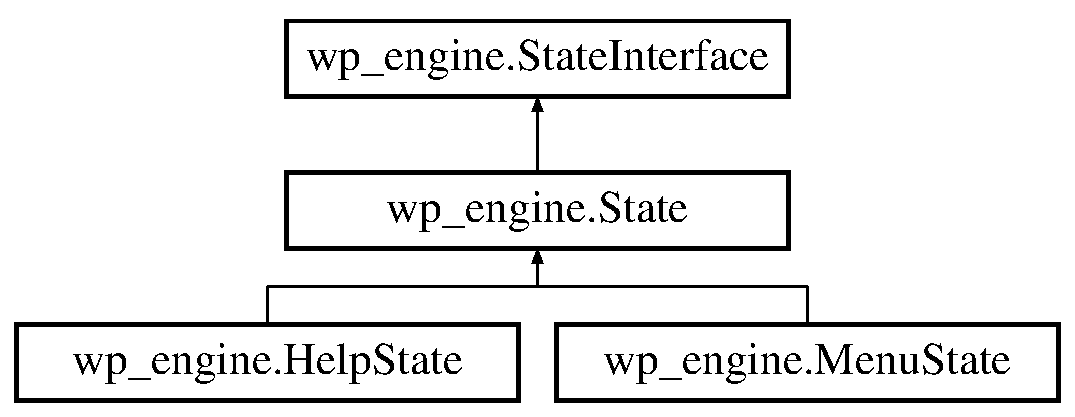
\includegraphics[height=3.000000cm]{interfacewp__engine_1_1_state_interface}
\end{center}
\end{figure}
\subsection*{Public Member Functions}
\begin{DoxyCompactItemize}
\item 
\hypertarget{interfacewp__engine_1_1_state_interface_a62e3b69584f695d55798b64ee98e738d}{void {\bfseries init} ()}\label{interfacewp__engine_1_1_state_interface_a62e3b69584f695d55798b64ee98e738d}

\item 
\hypertarget{interfacewp__engine_1_1_state_interface_ae1e1a65e47766241d880becba6c1a78b}{void {\bfseries update} (float elapsed\-Time)}\label{interfacewp__engine_1_1_state_interface_ae1e1a65e47766241d880becba6c1a78b}

\item 
\hypertarget{interfacewp__engine_1_1_state_interface_a1d96cd68833df5cd1520000801f123a1}{void {\bfseries load\-Content} (Content\-Manager content\-Manager)}\label{interfacewp__engine_1_1_state_interface_a1d96cd68833df5cd1520000801f123a1}

\item 
\hypertarget{interfacewp__engine_1_1_state_interface_a5157886c9fdcef20e5362c5a85503816}{void {\bfseries draw} (Sprite\-Batch sb)}\label{interfacewp__engine_1_1_state_interface_a5157886c9fdcef20e5362c5a85503816}

\end{DoxyCompactItemize}


\subsection{Detailed Description}
The inteface for game states. 

An advisory inteface.

Part of the state partition. 

The documentation for this interface was generated from the following file\-:\begin{DoxyCompactItemize}
\item 
State\-Interface.\-cs\end{DoxyCompactItemize}

\hypertarget{classwp__engine_1_1_state_manager}{\section{wp\-\_\-engine.\-State\-Manager Class Reference}
\label{classwp__engine_1_1_state_manager}\index{wp\-\_\-engine.\-State\-Manager@{wp\-\_\-engine.\-State\-Manager}}
}


A class that handles the states smoothly.  


\subsection*{Public Member Functions}
\begin{DoxyCompactItemize}
\item 
\hypertarget{classwp__engine_1_1_state_manager_ab3a0b2764d5f7c433ea193d5393a844e}{void {\bfseries add\-State} (\hyperlink{namespacewp__engine_aae123481cdcc6dc4c4474c1b0b62b152}{state\-Identifier} id, \hyperlink{classwp__engine_1_1_state}{State} state)}\label{classwp__engine_1_1_state_manager_ab3a0b2764d5f7c433ea193d5393a844e}

\item 
\hypertarget{classwp__engine_1_1_state_manager_ae14dcdb24376a69456d9bdb78687321b}{void {\bfseries update} (float elapsed)}\label{classwp__engine_1_1_state_manager_ae14dcdb24376a69456d9bdb78687321b}

\item 
\hypertarget{classwp__engine_1_1_state_manager_a5c86e0de0677343b27097ac605a1192c}{void {\bfseries draw} (Sprite\-Batch sb)}\label{classwp__engine_1_1_state_manager_a5c86e0de0677343b27097ac605a1192c}

\end{DoxyCompactItemize}


\subsection{Detailed Description}
A class that handles the states smoothly. 

Part of the state partition. 

The documentation for this class was generated from the following file\-:\begin{DoxyCompactItemize}
\item 
State\-Manager.\-cs\end{DoxyCompactItemize}

\hypertarget{classwp__engine_1_1_text}{\section{wp\-\_\-engine.\-Text Class Reference}
\label{classwp__engine_1_1_text}\index{wp\-\_\-engine.\-Text@{wp\-\_\-engine.\-Text}}
}


A class for text elements.  


\subsection*{Public Member Functions}
\begin{DoxyCompactItemize}
\item 
\hyperlink{classwp__engine_1_1_text_af3b9d3ba4bb3d3e589f7e32c02afd15c}{Text} (float x, float y, Sprite\-Font \hyperlink{classwp__engine_1_1_text_ac86929184c1426972dc3f0cdb768b3dc}{font}, string \hyperlink{classwp__engine_1_1_text_af48a92c9e88bc3c187ca8d807aa74cdd}{content})
\begin{DoxyCompactList}\small\item\em A constructor. \end{DoxyCompactList}\item 
\hyperlink{classwp__engine_1_1_text_af7139bad6c7931be5332e1efd2ed5a96}{Text} (\hyperlink{classwp__engine_1_1_object}{Object} target, Sprite\-Font \hyperlink{classwp__engine_1_1_text_ac86929184c1426972dc3f0cdb768b3dc}{font}, string \hyperlink{classwp__engine_1_1_text_af48a92c9e88bc3c187ca8d807aa74cdd}{content})
\begin{DoxyCompactList}\small\item\em A constructor. \end{DoxyCompactList}\item 
void \hyperlink{classwp__engine_1_1_text_aa8beb7b64ad8605ed1a0a2b3f602fa4f}{draw} (Sprite\-Batch sb)
\begin{DoxyCompactList}\small\item\em Draws the text. \end{DoxyCompactList}\end{DoxyCompactItemize}
\subsection*{Protected Attributes}
\begin{DoxyCompactItemize}
\item 
\hypertarget{classwp__engine_1_1_text_ac86929184c1426972dc3f0cdb768b3dc}{Sprite\-Font \hyperlink{classwp__engine_1_1_text_ac86929184c1426972dc3f0cdb768b3dc}{font}}\label{classwp__engine_1_1_text_ac86929184c1426972dc3f0cdb768b3dc}

\begin{DoxyCompactList}\small\item\em The font of the text. \end{DoxyCompactList}\item 
\hypertarget{classwp__engine_1_1_text_af48a92c9e88bc3c187ca8d807aa74cdd}{string \hyperlink{classwp__engine_1_1_text_af48a92c9e88bc3c187ca8d807aa74cdd}{content}}\label{classwp__engine_1_1_text_af48a92c9e88bc3c187ca8d807aa74cdd}

\begin{DoxyCompactList}\small\item\em The contents of the text. \end{DoxyCompactList}\end{DoxyCompactItemize}
\subsection*{Properties}
\begin{DoxyCompactItemize}
\item 
\hypertarget{classwp__engine_1_1_text_afdb55db0e26301ae2d0a7b049fc4c978}{Vector2 \hyperlink{classwp__engine_1_1_text_afdb55db0e26301ae2d0a7b049fc4c978}{location}\hspace{0.3cm}{\ttfamily  \mbox{[}get, set\mbox{]}}}\label{classwp__engine_1_1_text_afdb55db0e26301ae2d0a7b049fc4c978}

\begin{DoxyCompactList}\small\item\em Vector2 variable that stores the location of the object. \end{DoxyCompactList}\end{DoxyCompactItemize}


\subsection{Detailed Description}
A class for text elements. 

Part of the object partition. 

\subsection{Constructor \& Destructor Documentation}
\hypertarget{classwp__engine_1_1_text_af3b9d3ba4bb3d3e589f7e32c02afd15c}{\index{wp\-\_\-engine\-::\-Text@{wp\-\_\-engine\-::\-Text}!Text@{Text}}
\index{Text@{Text}!wp_engine::Text@{wp\-\_\-engine\-::\-Text}}
\subsubsection[{Text}]{\setlength{\rightskip}{0pt plus 5cm}wp\-\_\-engine.\-Text.\-Text (
\begin{DoxyParamCaption}
\item[{float}]{x, }
\item[{float}]{y, }
\item[{Sprite\-Font}]{font, }
\item[{string}]{content}
\end{DoxyParamCaption}
)\hspace{0.3cm}{\ttfamily [inline]}}}\label{classwp__engine_1_1_text_af3b9d3ba4bb3d3e589f7e32c02afd15c}


A constructor. 


\begin{DoxyParams}{Parameters}
{\em x} & the location of the text (x-\/coordinate) \\
\hline
{\em y} & the location of the text (y-\/coordinate) \\
\hline
{\em font} & the font of the text \\
\hline
{\em content} & the content of the text \\
\hline
\end{DoxyParams}
\hypertarget{classwp__engine_1_1_text_af7139bad6c7931be5332e1efd2ed5a96}{\index{wp\-\_\-engine\-::\-Text@{wp\-\_\-engine\-::\-Text}!Text@{Text}}
\index{Text@{Text}!wp_engine::Text@{wp\-\_\-engine\-::\-Text}}
\subsubsection[{Text}]{\setlength{\rightskip}{0pt plus 5cm}wp\-\_\-engine.\-Text.\-Text (
\begin{DoxyParamCaption}
\item[{{\bf Object}}]{target, }
\item[{Sprite\-Font}]{font, }
\item[{string}]{content}
\end{DoxyParamCaption}
)\hspace{0.3cm}{\ttfamily [inline]}}}\label{classwp__engine_1_1_text_af7139bad6c7931be5332e1efd2ed5a96}


A constructor. 


\begin{DoxyParams}{Parameters}
{\em target} & the object on which the text will be located \\
\hline
{\em font} & the font of the text \\
\hline
{\em content} & the content of the text \\
\hline
\end{DoxyParams}


\subsection{Member Function Documentation}
\hypertarget{classwp__engine_1_1_text_aa8beb7b64ad8605ed1a0a2b3f602fa4f}{\index{wp\-\_\-engine\-::\-Text@{wp\-\_\-engine\-::\-Text}!draw@{draw}}
\index{draw@{draw}!wp_engine::Text@{wp\-\_\-engine\-::\-Text}}
\subsubsection[{draw}]{\setlength{\rightskip}{0pt plus 5cm}void wp\-\_\-engine.\-Text.\-draw (
\begin{DoxyParamCaption}
\item[{Sprite\-Batch}]{sb}
\end{DoxyParamCaption}
)\hspace{0.3cm}{\ttfamily [inline]}}}\label{classwp__engine_1_1_text_aa8beb7b64ad8605ed1a0a2b3f602fa4f}


Draws the text. 


\begin{DoxyParams}{Parameters}
{\em sb} & the spritebatch of the game \\
\hline
\end{DoxyParams}


The documentation for this class was generated from the following file\-:\begin{DoxyCompactItemize}
\item 
Text.\-cs\end{DoxyCompactItemize}

%--- End generated contents ---

% Index
\newpage
\phantomsection
\addcontentsline{toc}{part}{Index}
\printindex

\end{document}
